\documentclass{report}
\usepackage{tikz}
\usepackage{graphicx} % Required for inserting images
\usepackage{tombstone}
\usepackage{hyperref}
\usepackage{minted}
\usepackage[a4paper, total={6in, 10in}]{geometry}
\usetikzlibrary{matrix}
% make numbering start from 1
\renewcommand{\thesection}{\arabic{section}}

% Set global options for minted
\setminted{
  frame=lines,
  framesep=2mm,
  baselinestretch=1.2,
  fontsize=\footnotesize,
  linenos
}

\setlength\parskip{0.7em plus 0.1em minus 0.2em}
\setlength\parindent{0pt}

\title{CS4215 Project Report}
\author{Jotham Wong A0235410W\\Arnav Aggarwal A0179505X}
\date{April 2024}
\bibliographystyle{plain}

\begin{document}

\graphicspath{{./images}}

\maketitle
\tableofcontents
\newpage

\section{Introduction}

\subsection{Report Goals}

This report aims to achieve the following:

\begin{enumerate}
    \item Outline scope and objectives of the project, including T diagrams of major language processing steps
    \item Give an informal specification of the language features and how they were implemented
    \item How we have achieved our baseline and stretch goals
    \item How to build and run the project
    \item Description of test cases
\end{enumerate}

\subsection{Ooga}

Ooga is a Concurrent Virtual Machine for a subset of the Go programming language. It implements an interpreter based on section 5.5 of Structure and Interpretation of Computer Programs, Javascript Edition (SICP JS). The source code for the interpreter can be found online at \url{https://github.com/CS4215-OOGA/ooga-lang} while the source code for the web editor can be found online at \url{https://github.com/CS4215-OOGA/ooga-frontend}.

All of the baseline expections in the term project outline have been achieved:

\begin{enumerate}
    \item Web-based implementation using Microsoft's Monaco Editor.
    \item An incrementally developed go language parser based on Pegjs
    \item Implementation uses a Compiler and Virtual Machine
    \item Sequential language constructs: variable and function declarations, blocks, conditionals, expressions and for loops
    \item Concurrent constructs: Go routines, concurrency control
    \item Low level memory model, and all runtime data structures are allocated from a single ArrayBuffer
\end{enumerate}

In addition to the baseline expectations, we have further achieved the following stretch goals

\begin{enumerate}
    \item Struct declarations
    \item Ability to declare standard library with custom types
    \item Type Safety and Type Checker
    \item Memory management with variable amount of nodes
    \item Lisp 2 Garbage Collection strategy
    \item Higher order functions
    \item Select statement
    \item Slices, buffered and unbuffered channels using make
    \item Visualization of runtime, operating, environment and heap in a graph view, with support for breakpoints
    \item Meaningful error messages in frontend
\end{enumerate}

\section{Language Processing Steps}

The Ooga tool-chain comprises a parser, compiler, typechecker and an interpreter, all written in Typescript. We use the open source library Peggy, which is a parser generator for Typescript, which takes in a pegjs grammar file and generates a javascript parser for the grammar as seen in Fig \ref{fig:ooga-parser-pegjs}. All typescript source files were first compiled to javascript.

\begin{figure}
    \centering
    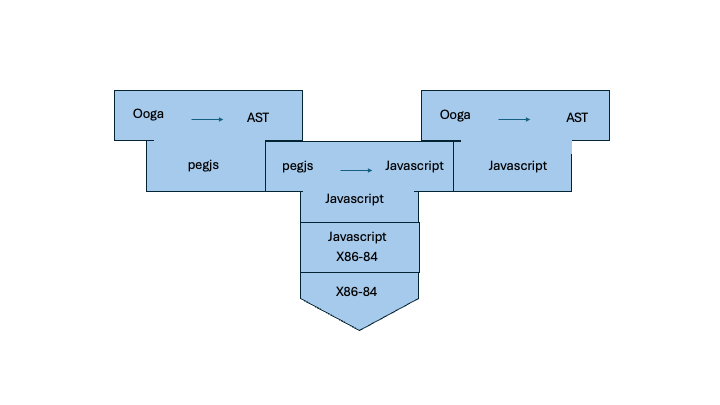
\includegraphics[width=1.25\linewidth]{ooga-parser-t-diagram.png}
    \caption{T-Diagram for Ooga-parser compilation}
    \label{fig:ooga-parser-pegjs}
\end{figure}

The language processing step for the main ooga-toolchain can be seen in Fig \ref{fig:ooga-toolchain}. We first parse the Ooga source code into an AST using the peggy generated parser. The AST is then compiled into Ooga bytecode using the Ooga compiler.

\begin{figure}
    \centering
    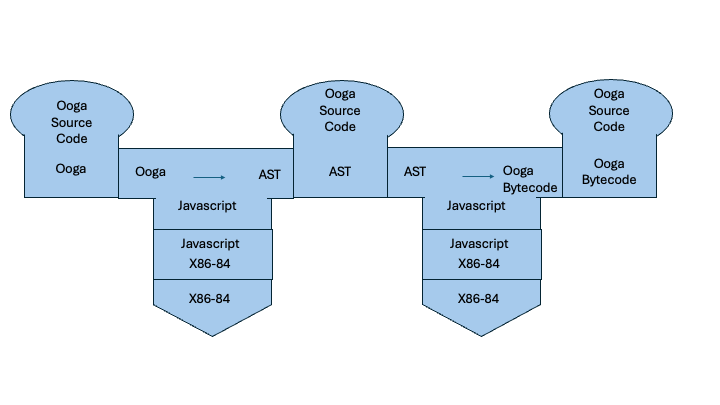
\includegraphics[width=1.25\linewidth]{ooga-compilation-t-diagram.png}
    \caption{T-Diagram for Ooga-compilation}
    \label{fig:ooga-toolchain}
\end{figure}

Finally, we run the Ooga bytecode using the Ooga-VM which acts as an interpreter.

\begin{figure}
    \centering
    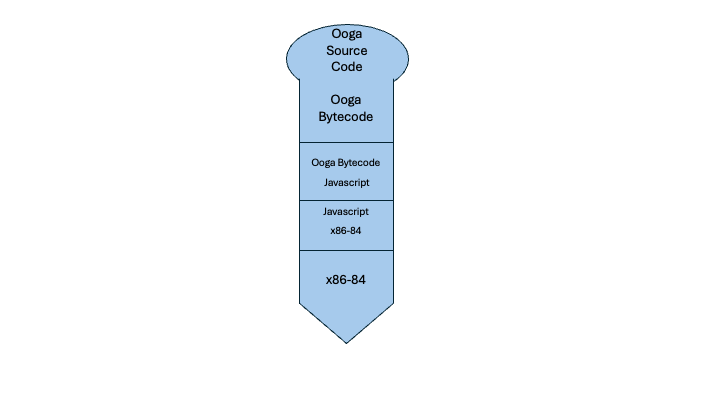
\includegraphics[width=1.3\linewidth]{ooga-vm-t-diagram.png}
    \caption{T-Diagram for running Ooga program with Ooga-VM}
    \label{fig:ooga-vm}
\end{figure}

\section{Parser}

The parser comprises of the Ooga pegjs grammar file and the Peggy generated parser file as seen in Figure \ref{fig:pegjs-pipeline}.

\begin{figure}
    \centering
    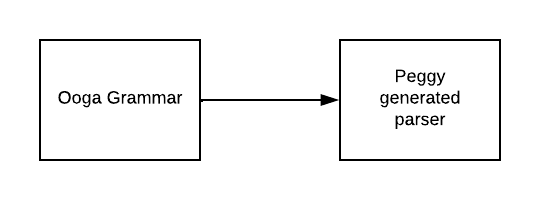
\includegraphics{pegjs-pipeline.png}
    \caption{Pipeline for pegjs parser}
    \label{fig:pegjs-pipeline}
\end{figure}

As there did not exist an open source pegjs grammar file for the Go programming language, we faced additional challenges in learning the pegjs grammar rules and in developing our own grammar for Go. The Ooga grammar was initially based on Peggy's public grammar for Javascript and modified to fit the language specifications of Go which Ooga is based on, and is stored at /src/parser/ooga.pegjs. As we only implemented a subset of the Go programming language, we added the minimal modifications necessary and removed all other grammar constructs that were not shared between javascript and Go.

With the ooga.pegjs grammar file, the Peggy parser code is generated using the 'yarn peggy' command and is stored in /src/parser/ooga.js. The parse function from peggy is exported for use by the Ooga toolchain. AST specific parser information will be discussed whenever appropriate.

\section{Typechecker}

The typechecker is the next component of the Ooga language. It ensures that the program is type-safe and can be executed without runtime type errors. The typechecker is implemented as a set of functions that traverse the Peggy-generated AST and perform type checking on each node. The main entry point is the \texttt{checkTypes} function, which takes the entire program as input and returns a copy of the program with all unknown types resolved.\\

The typechecker is designed to handle the various constructs of the Ooga language, including:
\begin{itemize}
    \item Primitive types: integers, floats, booleans, strings, and null
    \item Structured types: structs, arrays, and channels
    \item Function and method declarations
    \item Control flow statements: if, switch, for, and select
    \item Concurrency constructs: goroutines and channels
    \item Function calls (with overloading)
\end{itemize}

Ooga is a statically and strictly typed language, which means that all types are checked at compile-time before the program is executed. This allows the typechecker to perform thorough type analysis and catch any type-related errors early in the development process, rather than at runtime.\\

Additionally, the typechecker not only checks the types of the program, but also hydrates the types of all the items in the AST. This ensures that the compiler has access to the complete type information, which is particularly useful for constructs like structs, where the compiler needs to know the field positions and method signatures.

\subsection{Type Representation and Lookup}
Types are represented as instances of classes defined in \texttt{oogavm-types.js}, which includes:
\begin{itemize}
    \item Primitive types: \texttt{IntegerType}, \texttt{FloatType}, \texttt{BooleanType}, \texttt{StringType}, \texttt{NullType}.
    \item Structured types: \texttt{ArrayType}, \texttt{StructType}, \texttt{ChanType}.
    \item Function and method signatures: \texttt{FunctionType}, \texttt{MethodType}.
\end{itemize}

These types are utilised in the type environments, which are essentially linked lists of scope frames (each frame being a dictionary mapping variable names to types) that facilitate scope handling and type lookup.\\

Type lookup is performed using the \texttt{lookup\_type} function, which searches through a type environment (a linked list of dictionaries) to find the type associated with a given name. The type environment is divided into two parts: the \texttt{global\_type\_environment} and the \texttt{global\_struct\_environment}. The global type environment contains the types of built-in functions and operators, while the global struct environment contains the definitions of user-defined struct types.\\


\subsection{Overloaded Operators and Type Polymorphism}\label{section:typechecker-operators}

Ooga supports operator overloading, which allows operators such as the \texttt{+} to perform different operations based on the types of its operands. This feature is crucial for supporting polymorphism, where the same operation can adapt to different types, enhancing the language's flexibility and expressiveness.\\

The typechecker handles operator overloading by maintaining an array of \texttt{FunctionType} objects for each operator. Each \texttt{FunctionType} describes a valid combination of operand types and the resulting type after the operation. During type checking, the typechecker matches the operand types against these function types to select the appropriate operation.\\

For example, the \texttt{binary\_add\_type} array in the global type environment contains the type signatures for the \texttt{+} operator, allowing it to be used for both arithmetic operations and string concatenation:

\begin{minted}{javascript}
const binary_add_type = [
    new FunctionType([new StringType(), new StringType()], new StringType()),
    new FunctionType([new IntegerType(), new IntegerType()], new IntegerType()),
    new FunctionType([new FloatType(), new FloatType()], new FloatType()),
    new FunctionType([new IntegerType(), new FloatType()], new FloatType()),
    new FunctionType([new FloatType(), new IntegerType()], new FloatType()),
];
\end{minted}

This design enables the typechecker to support overloaded operators efficiently. Currently, overloading in Ooga is limited to built-in functions and operators. This limitation ensures that the type checking process remains manageable and avoids the complexity that user-defined overloaded functions might introduce.

\subsection{BlockStatement Typechecking}
The most complex part of the typechecker is the handling of \texttt{BlockStatement} nodes in the AST. These nodes represent a block of statements, such as the body of a function or the body of an if-statement. The typechecking process for a block statement is as follows:\\

1. \textbf{Struct Declarations}: First, the typechecker identifies all struct declarations in the block and adds them to the \texttt{global\_struct\_environment}. This allows for recursive struct definitions, as the type of the struct is available before its fields are processed.

2. \textbf{Known Type Declarations}: Next, the typechecker processes all variable, constant, function, and method declarations that have an explicit type. These are added to the \texttt{extended\_te} type environment, which is a copy of the current type environment with the new declarations.

\label{section:type-inference}
3. \textbf{Unknown Type Declarations}: After processing the known type declarations, the typechecker goes through any remaining variable or constant declarations that have an "unknown" type. For these, the typechecker infers the type from the expression being assigned to the variable or constant, and adds the inferred type to the \texttt{extended\_te} environment.

4. \textbf{Body Typechecking}: Finally, the typechecker recursively checks the type of the body of the block statement, using the \texttt{extended\_te} environment.

This order of operations is important because it allows the typechecker to handle recursive type definitions and resolve unknown types before checking the body of the block. It also ensures that variables and constants declared within the block have the correct type, even if they are used before their declaration.

\subsection{Function and Method Declarations}
The typechecking of function and method declarations is also quite complex, as it involves handling the return type and ensuring that the actual argument types match the expected argument types.

For function declarations, the typechecker first creates a \texttt{FunctionType} object that represents the type of the function. This includes the parameter types and the return type. It then extends the type environment with the parameter types, and recursively checks the body of the function. Finally, it ensures that the actual return type matches the expected return type.

For method declarations, the typechecker first checks that the receiver type is a valid struct type. It then creates a \texttt{MethodType} object that represents the type of the method, including the receiver type, parameter types, and return type. This method type is added to the struct type's list of methods.

\subsection{Concurrency Constructs} 
The typechecker also handles the concurrency constructs of the Ooga language, such as goroutines and channels. For goroutines, the typechecker simply checks that the expression being executed in the goroutine has a valid type.\\

For channels, the typechecker ensures that the type of the elements being sent or received matches the element type of the channel. It also checks the arguments to the \texttt{make} function when creating a new channel, ensuring that the buffer size (if provided) is an integer.

\subsection{Other Constructs}
The typechecker handles the remaining language constructs, such as arithmetic and logical expressions, conditional statements, and array and struct initializers, by recursively checking the types of the subexpressions and ensuring that they are compatible.\\

For example, in the case of a binary arithmetic expression, the typechecker first checks the types of the left and right operands. If they are both integers or both floats, it infers the appropriate return type. If the operands are of mixed types, it attempts to find a compatible function type in the global type environment.

\subsection{Error Handling}
Throughout the typechecking process, the typechecker may encounter type errors, such as a variable being used before it is declared, or an argument being passed to a function with an incompatible type. When such errors are encountered, the typechecker throws a \texttt{TypecheckError} exception, which contains information about the error, such as the expected and actual types. These error messages are then surfaced to the user, allowing them to debug and fix any type-related issues in their Ooga program.

\section{Memory Management}

The Ooga Virtual Machine uses a low-level memory model as well as a few high-level Javascript objects to implement the Ooga runtime.

\subsection{Memory Allocation}

One major limitation plaguing the toy programming language we learnt in CS4215 is the arbitrary node size of 10 words used to implement the heap. It makes garbage collection and memory allocation simple but it makes writing more interesting programs very difficult since each frame is only limited to 10 variable declarations.

We recognized this and decided to use a memory model that supported nodes of variable size. This was supported by changing the header format of each word. The first two words of each node is now the header and the third word onwards is the payload. The first four bytes of the node contains the size of the node in words and the next four bytes contains the tag of the node. The second word of the node contains the forwarding address of the node. Because our nodes are now variable size, a simple translation of the mark and sweep or copy garbage collection algorithm we learnt in class would not suffice. As such, we explored the different garbage collection strategies available and opted for the Lisp 2 mark-compact garbage collection due to its simplicity and performance.

Our heap contains a free variable that represents the current offset into the byte array that is free for allocation as well as a max variable to indicate the max length of the byte array. When we allocate a structure, we increment the free variable by the variable size of the node in words. 

Regardless of type, the first 2 words are reserved for header information. We assign the first word of the node to contain the variable's tag and size, and set the second word of the node to forward to its address. The subsequent words are type dependent and are elaborated below.

\subsection{Memory Format}

\subsubsection{Literals}

We pre-allocate the False, True, Null, Unassigned, Undefined and empty string (see later for Strings) literals onto the heap on machine initialization. They each occupy only 2 words and are identified only by their tag.

\subsubsection{Number}

Ooga supports floating point numbers only, with fake support for integers as our interpreting language is javascript. All numbers occupy 3 words, with the third word used for the number payload.

\subsubsection{Frames}

Block frames represent the frame bindings of values to names within the scope of a block and only occupy 3 words, with the third word used to store the address of the environment that the block frame points to.

Call frames occupy 4 words instead as they need to use the third word to store the return PC address (which is a number) and the fourth word to store the address of the environment.

Frames are the first truly variable sized nodes and occupy 2 + n words, where n is the number of binding names in the context. The third word onwards stores the address of each value in the frame.

\subsubsection{Closure}

Closures occupy 4 words. The arity is stored as a Uint8 at the 3rd word while the return PC address is stored as a Uint16 at the 3rd word at the first byte offset. This effectively means that the maximum length of our programs can only be 65536. For the purposes of our toy programming language, this would suffice and could trivially be changed to a Uint32 in future iterations. Finally, the address of the closure's environment is stored at the fourth word. 

\subsubsection{Environment} \label{section:env-node}

Environments can contain a variable number of frames, one for each level of nesting. When we extend an environment, we create a new environment with 1 + number of frames of the old environment, and copy each frame value accordingly before allocating the new frame to the latest frame value.

\subsubsection{Stack}\label{section:stack-node}

We support both the OS and RTS by using a Stack Node. The Stack Node occupies 4 words, with the third word being used to store the address of the previous Stack Node and the fourth word storing the address of the stack value. This effectively forms a stack data structure by recursively traversing the previous Stack address until a -1 is encountered, which indicates the end of the Stack.

\subsubsection{Builtins}

Builtins occupy 3 words, with the 3rd word being used to store the builtin identifier in the builtin mapping, in a similar manner to the toy programming language we used.

\subsubsection{Structs}

Ooga supports custom user-defined Structs by treating all Structs as a frame. Each attribute is indexed accordingly and the Struct is consequently treated as a frame by compile time frame look up. It consequently occupies 2 + numFields words.

\subsubsection{Strings}

Ooga supports String Pooling as covered in the homework by using a low level memory model to store the String literals as well as high level Javascript objects to implement the String Pooling.

At the byte level, Strings are treated as char ASCII arrays, with each char only occupying 1 byte. Thus, the number of words that a String occupies is the ceiling of the length of the String divided by 8. A String of length 9 would thus occupy 2 words for the char array payload. The third word of the Node is reserved to store the length of the String while the fourth word onwards store the payload.

At the high level, we maintain a mapping of Strings to addresses. When we allocate a String, we first check if we have already allocated the String using the map. If so, we simply return the address of the String, else we allocate the new String and return its address.

\subsubsection{Array and Slices}

Ooga supports both fixed size arrays and slices, which are dynamically resizable arrays. Arrays are equivalent in implementation to frames, so we elaborate on how slices are implemented.

In keeping with the Go language specifications, a slice stores its length, which is the current number of items that the slice stores, as well as its capacity, which is how much memory is allocated for the slice's contents. Slices and arrays both support indexing and index assignment but slices further support Go's append function which takes in a slice and a value and returns a slice with that value appended. When we append to a slice that has not met its capacity yet, the appending is trivial. However, when we append to a slice that has met its capacity, a new slice of double capacity is allocated onto the heap, the existing items in the old slice copied by address, the new item appended, and its address returned. We have added a test case in our test suite to demonstrate that Ooga behaves similarly to Golang in functionality, please refer to Section \ref{section:test-cases}.

\subsubsection{Channels}

Ooga supports both buffered and unbuffered channels. In keeping with the Go language specification, the channels are First-In-First-Out (FIFO) data structures. The details of the concurrency aspects of the channels will be delegated to Section \ref{section:channels}.

At the memory level, both buffered and unbuffered channels have an internal capacity which determine how many values they can store before becoming full and blocking. The unbuffered channel occupies 4 words (as it has a fixed capacity of 1) while the buffered channel occupies 3 words + capacity. Although an unbuffered channel is effectively a buffered channel with capacity 0, we use all bits in the header words and therefore it is more efficient to simply use the 3rd word to store a length instead of a boolean value. 

Consequently, both channels store their current length in the 3rd word and their payload in the 4th word onwards. To implement the FIFO mechanism, we push values onto the channel by appending to the last valid occupied word using the length variable. To pop values in a FIFO manner, we copy over the values from the 2nd element backwards, thus effectively deleting the first element and updating the length variable to account for the update. This O(N) approach was chosen due to its simplicity as we would otherwise have to allocate new nodes to represent the element of a channel which adds further complexity.

\subsection{Memory Access}

As the entire memory is implemented using one contiguous Javascript ArrayBuffer, all memory access only requires the word address of the node which serves as the byte offset from the start of the ArrayBuffer.

All memory access is first done by checking the tag of the memory node and then using the exposed methods to ensure that the right retrieval method is used, e.g. 32 bit unsigned integer vs a signed 16 bit integer vs a 64 bit floating number.

\subsection{Garbage Collection}

Due to the single contiguous nature in which we allocate memory, there will inevitably be garbage data as seen in Figure \ref{fig:garbage-data}.

\begin{figure}
    \centering
    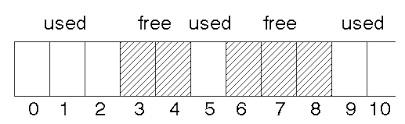
\includegraphics[width=0.5\textwidth]{memory-compaction.png}
    \caption{Garbage data}
    \label{fig:garbage-data}
\end{figure}

As our nodes are variable size, we cannot simply employ the same linked list pointer traversal as performed in the homework. Consequently, we have to perform memory compaction as seen in Figure \ref{fig:heap-compaction}.

\begin{figure}
    \centering
    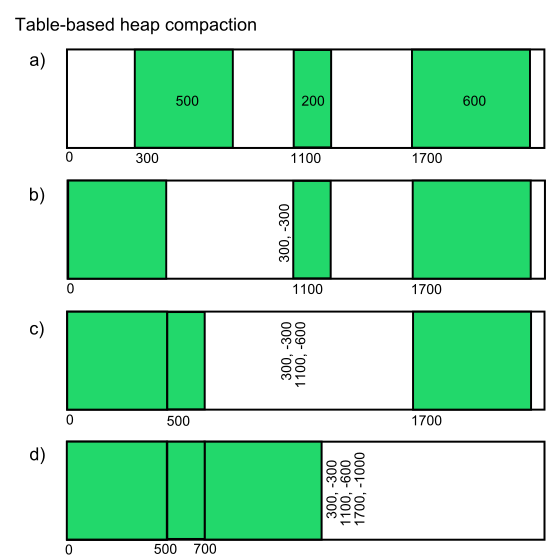
\includegraphics[width=0.5\textwidth]{table-compaction.png}
    \caption{Heap compaction}
    \label{fig:heap-compaction}
\end{figure}

We decided to implement the Lisp 2 GC algorithm due to its simplicitly and O(N) runtime. The Lisp 2 GC algorithm works by 4 linear sweeps over the heap. 

The first sweep marks live nodes in a similar manner to mark and sweep by starting from a set of root nodes which includes the literals and the Strings in the StringPool. This mark recursively visits the children of each node, such as each element in an array node or the value bindings of a frame node. At the end of the traversal, we have partitioned the heap into a set of live and dead nodes. As this is effectively mark and sweep, we will not run into issues with cyclical memory structures. We mark nodes by inverting the tag of the node, since all our tags are positive, this effectively identifies a live node from a dead node.

The second sweep computes the forwarding address for live objects. It does this by maintaining a free pointer and a live pointer and incrementing the live pointer through all nodes until it points to a live node. Thereafter, it updates the forwarding address (which is the second word) of the live node to the address of the current free pointer and then increments both the free pointer and the live pointer by the node's size. Because all garbage data has previously been initialized properly, the size is not garbage and correctly points to the next node, alive or not. 

The third sweep updates the pointers of each node to their corresponding forwarded addresses by linearly iterating through the heap. For example, nodes such as a block frame have an environment variable which now points to the current address of the environment but not its forwarded address (which would be its new address after compaction). These children pointers consequently need to be updated appropriately.

The fourth and final sweep moves the live objects to their forwarded addresses by copying each word of the object to its corresponding word offset at the forwarded address. This completes the memory compaction, and the free variable now points to the next offset of the heap that is free for allocation.

However, many complexities and potential bugs arise due to the segregation of the heap from our virtual machine when compaction GC is used. We previously used numbers to store the addresses of the allocated memory. However in cases where another allocation happens in the same function and garbage collection is triggered, the address now points to the incorrect address. We can understand this through an older (truncated) version of our CALL code as seen here

\begin{minted}{javascript}
    CALL: instr => {
        const arity = instr.arity;
        const fun = peekStackN(OS, arity);
        if (isBuiltin(fun)) {
            return applyBuiltin(getBuiltinID(fun));
        }
        let newPC = getClosurePC(fun);
        const newFrame = allocateFrame(arity);
        ...
        // Set newFrame values...
        ...
        let newCallFrame = allocateCallFrame(E, PC);
        RTS = pushStack(RTS, newCallFrame);
        ...
    },
\end{minted}

In our motivating example, after allocateCallFrame, if garbage collection triggers, the address that newFrame points to may now be garbage data. Since these variables are numbers, we cannot easily update them to their new forwarding addresses. 

To address this issue elegantly, we opted to store all memory addresses in arrays. Every time we allocate data onto the heap, we use arrays to store the current memory address, push these addresses onto our temporary roots and then perform the allocation. If garbage collection occurred, our arrays which are passed by reference and stored as temporary roots, will now correctly contain the forwarded memory address.

We also needed to update the roots in the virtual machine (which are arrays containing a single number), to their new forwarded address. We achieve this by storing a function with its closure to the roots of the virtual machine and updating their elements. We need to do this before the fourth sweep because otherwise the data at the root will now be garbage data and we have lost our machine's state.

This additional complexity is worth it however because our user programs can now support an arbitrary number of variable and function declarations which improve the developer experience of Ooga developers. Comprehensive test cases that demonstrate the correctness of our garbage collection and memory allocation can be found in Section \ref{section:test-cases}.

\section{Implementation of Language Features}

In this section, we dive into an overview of how the language features were implemented using the Ooga compiler and VM.

\subsection{VM State}

Our concurrent VM maintains the state of execution for a given program and a thread through the Operand Stack (OS), Program Counter (PC), Environment (E) and Runtime Stack (RTS) registers as well as a Javascript ByteArray to represent the low level memory heap. The OS, E and RTS registers are simply addresses in the heap as opposed to Javascript lists. OS and RTS point to a Stack Node in the heap while E points to an Environment Node in the heap.

To support the concurrency language features of Golang, our VM also uses additional state such as a TimeQuanta, a thread scheduler, a builtin mapping for builtin functions, which will have more elaboration in Section \ref{section:concurrency}.

\subsubsection{Operand Stack}

The Operand Stack is a stack of intermediate values represented as Stack Nodes \ref{section:stack-node} which can contain any kind of value. In Ooga, all expressions produce a value that are pushed onto the Operand Stack. More elaboration is provided in Section \ref{section:value-producing}.

\subsubsection{Runtime Stack}

The Runtime Stack is a stack of intermediate values represented as Stack Nodes \ref{section:stack-node} which can contain either CallFrame or BlockFrame nodes. The Runtime Stack is used so that Ooga can support closures for function calls which return to their proper addresses with their surrounding context as well as blocks which extend the current environment.

\subsubsection{Environment}

At runtime, the environment is a list of lists which are represented by Environment Nodes and Frame Nodes as detailed in \ref{section:env-node} which facilitates looking up the values of names as well as the assignment of values to names. At the implementation level, there are no more names stored in the environment due to our compile time lookup optimisation as detailed in \ref{section:cte-lookup}. At compile time, the environment is a Javascript list of lists instead to simplify development.

\subsection{Name Declarations and assignments}

Ooga supports 3 fundamental types of declarations - variable, constant and function declarations (more precisely function definitions).

Some supported declarations are shown below

\begin{minted}{go}
    var a int = 1; // variable decl and assignment with explicit typing
    b := 2; // variable decl and assign with implicit type inference
    var c string = "Jotham"; // string decl and assignment
    var d []int; // int slice decl
    e := make([]int, 5, 10); int slice decl and assignment
    const f = 1; // const decl with implicit type inference
    // f = 2; // will throw compile error

    func foo(a int, b int) int { // func declaration
        return a + b;
    }

    type Vector struct {
        x int
        y int
    }

    v := Vector{1, 1}; // decl and instantiation of a struct
\end{minted}

\subsubsection{Lexical scoping and name look up} \label{section:cte-lookup}

The following snippets of code will act as blocks

\begin{minted}{go}
// Treated as a block statement
var x int = 4;
{
    var x int = 5;
}
// So both values of x will exist in different frames

// The parameters will be treated as a separate frame
func foo(x int) { 
    var x int = 5; // this will also create another frame with x
}
\end{minted}

Our Virtual Machine makes use of the \textbf{Compile Time Environment look up optimisation} to speed up the look up of names at runtime. Firstly, when our parser encounters a pair of curly brackets or a list of parameters in a function call, it treats the current code block as a BlockStatement that wraps up a SequenceStatement.

At compilation time, we scan the block for Name Declarations (which include Variable, Constant and Function declarations) and push these declarations into a CompileTime Frame. We then append the CompileTimeFrame to the CompileTimeEnvironment. A slight optimisation is performed here, we do not append the CompileTimeFrame if it is empty - there are no new variable declarations.

\begin{minted}{javascript}
type CompileTimeVariable = {
    // This would be an object if it is a method 
    // - {receiver: string, methodName: string}
    name: string | Method;
    type: Type | null;
    is_const: boolean;
};
type CompileTimeFrame = CompileTimeVariable[];
type CompileTimeEnvironment = CompileTimeFrame[];
    
\end{minted}

Subsequent references to these names in the current block or nested block will find the latest frame index (indexed into the Environment list) and value index (indexed into the Frame list) by starting from the last frame and iterating backwards, as described in Chapter 5.5.6 of SICP JS. At this point, there are no longer any symbols associated with the declarations in the block. The tuple (frameIndex, valueIndex) are then pushed into the LD machine instruction. Upon exiting a block, the CompileTimeEnvironment pops off the latest CompileTimeFrame.

At runtime, when the current environment is extended, a block frame that contains the current environment is pushed onto the RTS. This allows us to restore the original environment when we exit the block. We then create a new environment with one more frame slot. We copy over the existing frame values of the old environment to the new environment, set the last frame to the frame for the current block and then update E to point to the newly allocated environment node. The VM's runtime Environment therefore corresponds 1 to 1 with the CompileTimeEnvironment at that point in time, and so all tuple look ups correctly match. When the VM encounters a LD machine instruction, it will look up its current E by indexing into the Environment using the machine level interface to retrieve the corresponding value. 

\subsubsection{Variable Declarations and Assignments}

We support both styles of Golang variable declarations as seen below

\begin{minted}{go}
    var x int; // declaration
    y := 5;    // implicit type inference and assignment
    var z int = 5; // explicit type inference and assignment
\end{minted}

However, we do not support multiple variable declarations on the same line, so expressions such as 

\begin{minted}{go}
    var i, j int = 1, 2;
\end{minted}

are not supported.


Variable declarations are parsed by pegjs as 

\begin{minted}{javascript}
VariableStatement
    = VarToken __ id:Identifier __ typeInit:(TypeWithInit)? EOS {
        return {
            tag: "VariableDeclaration",
            id: id,
            expression: typeInit.init ? extractOptional(typeInit.init, 1) : null,
            type: typeInit.type || "Unknown"
        }
    }
    / VarToken __ id:Identifier __ typeInit:(TypeWithoutInit)? EOS {
        return {
            tag: "VariableDeclaration",
            id: id,
            expression: null,
            type: typeInit.type || "Unknown"
        }
    }
    / id:Identifier init:(__ ShorthandInitialiser) EOS {
        return {
            tag: "VariableDeclaration",
            id: id,
            expression: extractOptional(init, 1),
            type: "Unknown",
            shorthand: true
        }
    }
    / id:Identifier init:(__ ShorthandStructInitializer) EOS {
        return {
            tag: "VariableDeclaration",
            id: id,
            expression: extractOptional(init, 1),
            type: "Unknown",
            shorthand: true
        }
    }
\end{minted}

Our parser transforms these expressions into VariableDeclaration components which comprise of an id, expression and a type. Observe that some of the types are treated as "Unknown", these will automatically be inferred by our typechecker as elaborated in \ref{section:type-inference}. Furthermore, observe that we allow the expression to be null to allow statements such as 

\begin{minted}{go} 
    var x int; 
\end{minted}

In this case we use the following default initialization strategy.

\begin{enumerate}
    \item Integers and Floats are assigned a default value of 0.
    \item Booleans are assigned a default value of false.
    \item Strings are assigned a default '' empty string value.
    \item Non-primitive types such as arrays and channels are assigned a default value of null.
    \item Structs have their non struct fields default initialized and struct fields initialized to null.
\end{enumerate}

To illustrate default initialization of Structs, refer to this code snippet

\begin{minted}{go}
    type Node struct {
        value int
        flag bool
        child Node
    }
    
    var n Node;
    
    print(n.value); // will print 0
    print(n.flag);  // will print false
    print(n.child); // will print nil
    
\end{minted}

\subsubsection{Function Declarations}

Function declarations are the other type of declarations in Ooga. To support goroutines, we support both named function declarations as well as anonymous function declarations as seen in the following code snippet.

\begin{minted}{go}
    // named function declaration without return
    func goo(x int) {
        // returns nothing
    }
    // named function declaration with return type
    func foo(x int) int { 
        return x;
    }
    // anonymous function to support goroutine
    go func(x int) { 
        print(x);
    }(5);
    
\end{minted}

Function declarations are parsed by pegjs as 

\begin{minted}{javascript}
LambdaDeclaration
  = FunctionToken __ "(" __ params:(FormalParameterList __)? ")" __
    "("? __ type:(ReturnType)? __ ")"? __
    "{" __ body:FunctionBody __ "}"
    {
      return {
        tag: "LambdaDeclaration",
        params: optionalList(extractOptional(params, 0)),
        ret: {type:type || "Null"},
        type: "Function",
        body: body
      }
    }

FunctionDeclaration
  = FunctionToken __ id:Identifier __
    "(" __ params:(FormalParameterList __)? ")" __
    "("? __ type:(ReturnType)? __ ")"? __
    "{" __ body:FunctionBody __ "}"
    {
      return {
        tag: "FunctionDeclaration",
        id: id,
        params: optionalList(extractOptional(params, 0)),
        ret: {type: type || "Null"},
        type: "Function",
        body: body
      };
    }

FunctionExpression
  = FunctionToken __ id:(Identifier __)?
    "(" __ params:(FormalParameterList __)? ")" __
    "("? __ type:(ReturnType)? __ ")"? __
    "{" __ body:FunctionBody __ "}"
    {
      return {
        tag: "LambdaDeclaration",
        id: extractOptional(id, 0),
        params: optionalList(extractOptional(params, 0)),
        body: body,
        ret: {type:type || "Null"},
        type: "Function"
      };
    }

FormalParameterList
  = head:FormalParameter tail:(__ "," __ FormalParameter)* {
      return buildList(head, tail, 3);
    }

FormalParameter
  = id:Identifier __ type:InitType {
      return { tag: id.tag, name: id.name, type: type };
    }
    / id:Identifier __ type:StructIdentifier {
      return { tag: id.tag, name: id.name, type: type };
    }

ReturnType
  = type:InitType {
    return type;
  }
  / type:StructIdentifier {
    return type;
  }
\end{minted}

Similar to the lecture material, we treat function declarations as syntatic sugar for constant assignments to lambda declarations. This allows us to treat functions as expressions themselves, which allows us to easily support higher order functions and goroutines.

\subsubsection{Handling assignment}

Consequently, when the compiler processes a VariableDeclaration, ConstantDeclaration or LambdaDeclaration component, it either compiles the component's expression or it compiles the variable's default initialization. It then looks up the symbol's Compile Time Position in the CompileTimeEnvironment and pushes a ASSIGN opcode alongside it's position.

At runtime, the VM will first evaluate the expression and push its memory address onto the OS. When it encounters the ASSIGN opcode, it sets the corresponding environment and frame index to that address. Note that the ASSIGNMENT instruction does not pop from the OS, this thus remains consistent with our notion that all statements are value producing.

\subsubsection{Handling constants}

Names that are treated as a constant have their flag is\_const set to true at the typechecker and compilation time. When the compiler encounters an assignment or update expression, it checks if the CompileTimeVariable's const flag is set to True, returning a compilation error if so.

\subsection{Builtins}

Our interpreted language makes use of builtin functions from our interpreting language (Javascript) in a similar manner to the Source toy language.

A mapping of function names to their implementations are stored in the constant builtinMappings in the oogavm-machine.ts file, which includes builtin functions such as print (which delegates to Javascript's console.log), start/endAtomic and getTime (used to implement time.Sleep).

Because we employ a compilation and interpreting (VM) phase, builtins are referenced in both phases and thus require special treatment. At compilation time, the builtinArray is populated with the names of each builtin function and initialized as the globalCompileTimeEnvironment. Subsequent function calls will reference their CompileTime position. At runtime, each builtin function is allocated onto the heap with its unique builtin-id and tag. When a Function Call is made, the VM would index the CompileTime position and acquire the memory address of the builtin function, checks that it is indeed a builtin function and call the appropriate value of the builtin mapping.

A sample of builtin functions is shown below:

\begin{minted}{javascript}
export const builtinMappings = {
    print: () => {
        let value: any;
        log('print sys call');
        [OS[0], value] = popStack(OS[0]);
        // need to handle the string 
        // representation of nil differently
        if (isNull(value)) {
            console.log('nil');
            return value;
        }
        console.log(addressToTSValue(value));
        return value;
    },
    ...
    getTime: () => {
        // Get unix time in millis
        return TSValueToAddress(Date.now());
    },
    ...
};
    
\end{minted}

\subsection{Binary, logical and unary operators}

Expressions that are supported by Ooga include all complex binary, logical and unary operations with typechecking done by our typechecker as discussed in Section \ref{section:typechecker-operators}.

\begin{minted}{go}
func foo(x int) int {
    return x + 5;
}

// complex boolean and arithmetic expression
((5 + foo(5)) * (10 - foo(4))) > foo(42);
"Ooga" + " " + "Booga!" // string concatenation
5++; // update expression
\end{minted}

\subsubsection{Parser}

Expressions involving binary, logical, and unary operations are parsed through a structured approach that deconstructs expressions into their constituent components: the left-hand side (LHS), the operator, and, for binary operations, the right-hand side (RHS). This methodology allows for precise interpretation and compilation of expressions.

\textbf{Binary and Logical Operators:} For operations such as arithmetic calculations or logical comparisons, the parser follows the format 'LHS operator RHS'. Here, 'LHS' and 'RHS' represent the operands, while 'operator' denotes the binary function (e.g., \texttt{+}, \texttt{-}, \texttt{*}, \texttt{/}, \texttt{\&\&}, \texttt{||}) applied to these operands. The parsing sequence involves processing the LHS first, followed by the operator, and then the RHS. This order of operations ensures that the operands are pushed onto the stack in the correct sequence for subsequent evaluation by the virtual machine.

\textbf{Unary Operators:} Unary operations, such as negation or logical NOT, are recognized in the format 'operator RHS'. In these expressions, the operator precedes the operand directly, and there is no LHS component. The operand is processed first, with the operator applied immediately afterward, allowing for efficient handling of unary operations.

\textbf{Implementation Details:} During the syntactic analysis phase, the parser treats LHS, operator, and RHS as separate elements. Recursive descent parsing techniques are utilized to handle subexpressions, particularly useful in managing nested operations. This parsing strategy ensures that operations are correctly grouped and ordered according to precedence and associativity rules defined in the language specifications.

At compilation time, our compiler recursively compiles the left side expression, then right side expression and finally pushes either the BINOP, UNARY or LOG opcode with the operator symbol. The compilation terminates eventually because the expressions will terminate in either literal values or name tagged components. The final result is that the AST will be evaluated by the VM in postfix order.

At runtime, the VM will either push literal values or look up the value of names and push their values onto the OS. It is important to note that because of our low level memory model, we actually allocate memory onto the heap that represents the javascript value of the expression and then push a Stack Node containing the value and the previous OS address onto the heap before updating our OS state. When it encounters an operator symbol such as "+", it pops the appropriate number of Stack Nodes from the OS, converts the memory addresses to javascript values, and then computes them using javascript. In this manner, we are able to support all javascript operations such as arithmetic and string concatenation.

\subsection{Sequence Statements}\label{section:value-producing}

In Ooga, all expressions are value producing and push a value onto the OS. We therefore handle Sequence statements by compiling each statement and inserting a POP machine code for every statement except the last statement. The value of a SequenceStatement is therefore the value produced by the last statement. Empty SequenceStatements instead push Undefined onto the OS.

\begin{minted}{go}
var x int = 5; // produces 5
// a POP is here
x + 5; // produces 10
// a POP is here
x + 10; // produces 15
\end{minted}

\subsection{Control Flow}

Ooga supports if, switch and for statements with break and continue.

\subsubsection{If statements}

If, if else and complex if else if statements are handled elegantly by the following pegjs grammar:

\begin{minted}{javascript}
IfStatement
  = IfToken __ test:Expression __
    consequent:Statement __
    ElseToken __
    alternate:Statement
    {
      return {
        tag: "IfStatement",
        test: test,
        consequent: consequent,
        alternate: alternate
      };
    }
  / IfToken __ test:Expression __
    consequent:Statement {
      return {
        tag: "IfStatement",
        test: test,
        consequent: consequent,
        alternate: { tag: "SequenceStatement", body: [] }
      };
    }
\end{minted}

Because an IfStatement is itself a Statement, subsequent else if statements are nested under the alternate expression of the first if statement, which evaluates recursively.

At compilation time, the compiler compiles the predicate and then pushes a Jump On False instruction that skips the consequent if the predicate evaluated to false. After the consequent's body, a GOTO instruction that jumps past the alternate is inserted. Because we treat consequent if elses as a nested alternate, we effectively jump over everything else if the consequent was true and recurse if it was false.

Maintaining consistency with our language semantics, if statements produce the value of their evaluated consequent or alternate.

\subsubsection{Switch statements}

Switch statements in Go have implicit breaks in each case and because we do not support fallthroughs, we are thus able to treat a SwitchStatement the same as an If Statements with the exception that our compiler inserts an equality test for the case's expression and the SwitchCase's discriminant component. Default switch cases simply have a null test and will always evaluate, if present.

\begin{minted}{javascript}
SwitchStatement
  = SwitchToken __ "("? __ discriminant:Expression __ ")"? __
    cases:CaseBlock
    {
      return {
        tag: "SwitchStatement",
        discriminant: discriminant,
        cases: cases
      };
    }

CaseBlock
  = "{" __ clauses:(CaseClauses __)? "}" {
    // Add a default case if none is present
    return optionalList(extractOptional(clauses, 0))
        .concat(
            {
                tag: "SwitchCase",
                test: null,
                consequent: {tag: "BlockStatement", body: []}
            }
        );
  }
  / "{" __
    before:(CaseClauses __)?
    default_:DefaultClause? __ "}"
    {
      return optionalList(extractOptional(before, 0))
        .concat(default_);
    }

CaseClauses
  = head:CaseClause tail:(__ CaseClause)* { return buildList(head, tail, 1); }

CaseClause
  = CaseToken __ test:Expression __ ":" consequent:(__ StatementList)? {
    return {
      tag: "SwitchCase",
      test: test,
      consequent: {tag:'BlockStatement', body: optionalList(extractOptional(consequent, 1))}
    };
  }

DefaultClause
  = DefaultToken __ ":" consequent:(__ StatementList)? {
    return {
      tag: "SwitchCase",
      test: null,
      consequent: {tag:'BlockStatement', body: optionalList(extractOptional(consequent, 1))}
    };
  }
\end{minted}

Note that our typechecker has already checked that the types of the case and the discriminant match. Our compiler then compiles each case separately, inserting a GOTO instruction at the end of each body that jumps to the end of all compiled cases.

 Something interesting of note is that we always insert a default switch case if it does not exist. This is to ensure that our switch statement always returns a value, which is useful for programs where a switch statement is used in a function which does not have a default return statement, such as the following

 \begin{minted}{go}
 func foo(x int) int {
    switch (x) {
        case 1:
            return 1;
    }
}
\end{minted}

Because we force an empty default switch case that returns null, our switch statement will always return a value and so the typechecker will throw a compilation error here.

\subsubsection{For loops}

For loops in Go are complex because they have 3 components: the initialization, predicate and update component which are all optional.

We handle this in the parser as follows:

\begin{minted}{javascript}
ForStatement
  = ForWithInitTestUpdate
  / ForWithTest
  / ForInfinite

ForWithInitTestUpdate
  = ForToken __
    init:ForInitStatement ";" __
    test:ForTest ";" __
    update:Expression __
    body:BlockStatement __
    {
      return {
        tag: "ForStatement",
        type: "ForWithInitTestUpdate",
        init: init,
        test: test,
        update: update,
        body: body
      };
    }


ForWithTest
  = ForToken __
    test:ForTest __
    body:BlockStatement __
    {
      return {
        tag: "ForStatement",
        type: "ForWithTest",
        init: null,
        test: test,
        update: null,
        body: body
      };
    }


ForInfinite
  = ForToken __
    body:BlockStatement __
    {
      return {
        tag: "ForStatement",
        type: "ForInfinite",
        init: null,
        test: { tag: "Boolean", value: true },
        update: null,
        body: body
      };
    }

ForInitStatement
  = VarToken __ id:Identifier __ type:(InitType) init:(__ Initialiser) {
        return {
            tag: "VariableDeclaration",
            id: id,
            expression: extractOptional(init, 1),
            type: type
        }
    }
    / id:Identifier init:(__ ShorthandInitialiser) {
        return {
            tag: "VariableDeclaration",
            id: id,
            expression: extractOptional(init, 1),
            type: "Unknown"
        }
    }
\end{minted}

Getting the grammar to work for the optional components alongside the TypeChecker was surprisingly more challenging than expected, thus we opted to handle all cases explicitly with the types manually filled in, as seen from the code above.

During compilation, we compile the Init component if it exists, extending the current environment with an enter scope if there exists a variable declaration within the init component.

We handle loop breaks and continues by inserting a loop marker at the start of the loop which keeps track of break and continue instructions. We then compile the test (predicate) component of the for loop if it exists and push a JOF instruction. We then compile the body of the ForStatement and insert a POP instruction afterwards, to prevent the value of the body from overwhelming the OS. ForStatements in Ooga thus return the value of their Predicate condition, if present, since that is the last component evaluated before the loop is exited.

If a Continue Statement had been encountered in the body of the ForStatement, we make the instruction jump to the Update component of the loop, if it exists. If there is no Update component, the Continue Statement jumps back to the Test component. In the case where both the Update and Test components are absent, the Continue Statement effectively jumps to the beginning of the loop body.

If a Break Statement is encountered within the body of the ForStatement, we insert a GOTO instruction that jumps to the end of the loop, effectively terminating the loop's execution. The loop marker ensures that the Break Statement is associated with the correct loop, allowing for proper handling of nested loops. When the Break Statement is executed, the program flow jumps to the instruction immediately following the loop's body, continuing with the next statement after the loop.

We then compile the Update component of the ForStatement, if present, and add a GOTO instruction that jumps back to the start of the loop, i.e., after the Init component. This ensures that the Update component is executed at the end of each iteration before the next iteration begins.

Finally, we insert an EXIT SCOPE instruction only if an ENTER SCOPE was inserted through the ForInit component. This is done to maintain the proper scoping of variables declared within the Init component and ensure that they are accessible only within the loop body.

By handling the optional components of the for loop and properly managing the flow of execution using JOF, GOTO, and EXIT SCOPE instructions, we ensure that the loop behaves as expected and maintains the correct scoping of variables throughout its execution.

\subsection{Structs}

Ooga supports the declaration and usage of custom struct types, allowing developers to define complex data structures with associated methods. This section explains the implementation details of structs, including struct declarations, struct initializers, and struct methods.

\subsubsection{Struct Declarations}

Ooga's struct declarations follow a syntax similar to Go, using the \texttt{type...struct} keyword. The parser handles struct declarations using the following grammar rules:

\begin{minted}{javascript}
StructDeclaration
  = TypeToken __ id:Identifier __ StructToken __ "{" __ fields:StructFieldList? __ "}" {
      return {
        tag: "StructDeclaration",
        id: id,
        fields: fields || []
      };
    }

StructFieldList
  = head:StructField tail:(__ StructField)* {
      return buildList(head, tail, 1);
    }

StructField
  = id:Identifier __ type:InitType EOS {
      return { tag: "StructField", name: id, type: type };
    }
    / id:Identifier __ type:StructIdentifier EOS {
        return { tag: "StructField", name: id, type: type };
    }
\end{minted}

During parsing, struct declarations are transformed into \texttt{StructDeclaration} AST nodes, containing the struct identifier (\texttt{id}) and an array of \texttt{StructField} objects representing the struct's fields. Each \texttt{StructField} object includes the field name (\texttt{name}) and its corresponding type (\texttt{type}).

To handle struct declarations during typechecking, we introduce a separate struct type environment (\texttt{struct\_te}). When the typechecker encounters a \texttt{StructDeclaration} node in the AST, it checks if the struct name already exists in the current struct type environment frame, throwing a \texttt{TypecheckError} if a redeclaration is detected. A new \texttt{StructType} object is created with the struct name and an empty array of fields, serving as a placeholder for the struct type. The struct name and its corresponding \texttt{StructType} object are added to the current block's struct type environment frame using the \texttt{extend\_current\_type\_environment} function.

The typechecker then iterates over the struct's fields and constructs \texttt{StructField} objects for each field. The field types are obtained by calling the \texttt{getType} function with the field's type node and the current struct type environment. The constructed \texttt{StructField} objects are assigned to the \texttt{fields} property of the \texttt{StructType} object, completing the struct type definition.

By maintaining a separate struct type environment, we ensure that struct types are properly registered and can be referenced within the same block scope. This allows for the declaration of struct types that contain fields of other struct types, enabling the creation of complex data structures.

The separation of the struct type environment from the regular type environment is necessary because it allows for the resolution of struct types before they are used in variable or function declarations. This way, when the typechecker encounters a reference to a struct type, it can retrieve the corresponding \texttt{StructType} object from the struct type environment and use it for type checking.

\subsubsection{Struct Initializers}

Ooga supports the initialization of struct values using struct initializers, which allow the creation of new struct instances with specific field values. The parser handles struct initializers using the following grammar rules:

\begin{minted}{javascript}
Struct
    = type:StructIdentifier __ "{" __ fields:StructFieldInitializerList? __ "}" {
        return { tag: "StructInitializer", fields: fields || [], named: true, type: type };
    }
    / type:StructIdentifier __ "{" __ values:StructValueInitializerList? __ "}" {
        return { tag: "StructInitializer", fields: values || [], named: false, type: type };
    }

StructInitializer
  = "=" !"=" __ struct:Struct {
      return struct;
    }
    / "=" !"=" __ expression:AssignmentExpression { return expression; }

ShorthandStructInitializer
  = ":=" __ struct:Struct {
      return struct;
    }

StructFieldInitializerList
  = head:StructFieldInitializer tail:(__ "," __ StructFieldInitializer)* {
      return buildList(head, tail, 3);
    }

StructFieldInitializer
  = id:Identifier __ ":" __ value:AssignmentExpression {
      return { tag: "StructFieldInitializer", name: id, value: value };
    }

StructValueInitializerList
  = head:AssignmentExpression tail:(__ "," __ AssignmentExpression)* {
      return buildList(head, tail, 3);
    }
\end{minted}

The parser supports both named field initializers (\texttt{StructFieldInitializerList}) and positional field initializers (\texttt{StructValueInitializerList}). 

During typechecking, the \texttt{StructInitializer} nodes are processed by first checking if the struct type exists in the \texttt{struct\_te}. If it exists, the typechecker retrieves the type and performs preliminary checks, matching the number of arguments received to the number of fields in the struct type.

For named field initializers, the typechecker iterates over the \texttt{fields} array and ensures that each field name exists in the struct type. If a field with the specified name is not found, a \texttt{TypecheckError} is raised. The field value expressions are then typechecked using the \texttt{type} function, and the resulting types are compared with the expected field types defined in the struct.

For positional field initializers, the typechecker iterates over the \texttt{fields} array and typechecks each value expression using the \texttt{type} function. The resulting types are then compared with the corresponding field types defined in the struct, in the order they appear.

During compilation, the compiler generates instructions to allocate memory for a new struct instance and initialize its fields based on the provided field values. The compilation process for struct initializers begins with the compiler emitting a \texttt{NEW\_STRUCT} instruction, specifying the struct type and the number of fields. This instruction allocates memory for the struct instance on the heap.

For each field initializer (named or positional), the compiler generates instructions to evaluate the field value expression and push the result onto the stack. After evaluating each field value, the compiler emits an \texttt{INIT\_FIELD} instruction, specifying the field index. This instruction pops the field value from the stack and initializes the corresponding field of the struct instance.

By following this compilation process, the compiler ensures that the necessary instructions are generated to create a new struct instance with the provided field values.

\subsubsection{Struct Methods}

Ooga also supports the declaration of methods associated with struct types, allowing developers to define behavior specific to struct instances. The parser handles method declarations using the following grammar rules:

\begin{minted}{javascript}
MethodDeclaration
  = FunctionToken __ "(" __ receiver:Receiver __ ")" __ id:Identifier __
    "(" __ params:(FormalParameterList __)? ")" __
    "("? __ type:(ReturnType)? __ ")"? __
    "{" __ body:FunctionBody __ "}"
    {
      return {
        tag: "MethodDeclaration",
        receiver: receiver,
        id: id,
        params: optionalList(extractOptional(params, 0)),
        ret: {type: type || "Null"},
        type: "Method",
        body: body
      };
    }

Receiver
    = id:Identifier __ "*" __ type:StructIdentifier {
        return { tag: "Receiver", name: id, type: type, pointer: true };
    }
    / id:Identifier __ type:StructIdentifier {
        return { tag: "Receiver", name: id, type: type, pointer: false };
    }
\end{minted}

During typechecking, the \texttt{MethodDeclaration} nodes are processed by retrieving the \texttt{StructType} object corresponding to the receiver's type from the struct type environment. A new \texttt{MethodType} object is created with the method name, parameter types, return type, and a boolean indicating whether the receiver is a pointer receiver. The \texttt{MethodType} object is then added to the \texttt{methods} array of the \texttt{StructType} object, associating the method with the struct type.

The method body is typechecked using the \texttt{type} function, treating the method as a regular function declaration. The receiver is added as the first parameter in the type environment. By associating methods with struct types, the typechecker ensures that methods can only be called on instances of the corresponding struct type and that the receiver type is correctly bound to the method.

During compilation, methods are treated similarly to regular functions, with a few key differences. The compiler generates a unique name for the method by combining the struct type name and the method name, ensuring that method names are properly mangled and avoid naming conflicts. The receiver is treated as an implicit first parameter of the method, and the compiler generates instructions to push the receiver instance onto the stack before pushing the method arguments.

The compiler generates a \texttt{CALL} instruction with an arity that includes the receiver instance, ensuring that the method is called with the correct number of arguments, including the receiver. Inside the method body, the compiler treats the receiver as a regular parameter, allowing access to its fields and methods using the \texttt{MemberExpression} syntax.

By following this compilation process, the compiler ensures that methods are properly associated with their corresponding struct types and that method calls are correctly handled at runtime.

An example of a method declaration is as follows:

\begin{minted}{go}
func (v *Vertex) AddX(x int) {
    v.x = v.x + x;
}
\end{minted}

We make use of the pointer notation, even though we do not currently support pointers, to reflect that all variables in Ooga are passed by reference instead of value.

\subsubsection{Method Calls}

Method calls in Ooga are handled similarly to regular function calls, with a few key differences. The parser handles method calls using the \texttt{CallExpression} grammar rule, where the callee is a \texttt{MemberExpression}.

When a \texttt{MemberExpression} is encountered during typechecking and the property is a method, the typechecker retrieves the corresponding \texttt{StructType} object and checks if the method exists in the struct's method list. If the method is not found, a \texttt{TypecheckError} is raised.

The compilation process for method calls involves several steps. The compiler generates instructions to evaluate the struct expression (\texttt{MemberExpression.object}) and push the struct address onto the stack. It then compiles the method arguments, pushing their values onto the stack. Finally, the compiler emits a \texttt{CALL} instruction with an arity that includes the receiver instance and the method arguments.

Here's an example of a method call in Ooga:

\begin{minted}{go}
var v Vertex = Vertex{1, 2};
v.AddX(3);
\end{minted}

In this example, \texttt{v} is an instance of the \texttt{Vertex} struct, and \texttt{AddX} is a method associated with the \texttt{Vertex} struct. The method call \texttt{v.AddX(3)} is compiled into instructions that push the struct address and the argument onto the stack, and then invoke the method using the \texttt{CALL} instruction.

The compilation of method calls ensures that the receiver instance is properly passed as an implicit first argument, allowing the method to access and modify the struct's fields.

\subsection{Slices and Arrays}

Slices and arrays are both supported and instantiated similarly to Go. Slices are instantiated via the make command while arrays are instantiated C-style.

\begin{minted}{go}
var x [5]int = [5]int{1, 2, 3, 4, 5}; // an array of size 5
len(x); // prints 5

// create a slice of len 5 and capacity 10
var y []int = make([]int, 5, 10); 
len(y); // prints 5
\end{minted}

Slices and arrays both share the same type declaration and are differentiated from one another by the TypeChecker. At compilation time, the array expression is compiled element by element, followed by a LDARR instruction which takes in the length of the element. At runtime, each expression is evaluated, pushed onto the OS and then used to populate the newly allocated array of provided length. On the other hand, slices are default initialized with the hydrated type from the typechecker.

Slice and array indexing and assignment are trivially handled by compiling the index expression and then the slice or array expression. At runtime, the appropriate indexing method exposed from the heap is called which pushes the value onto the stack. If there is an index out of bounds error, an error is thrown. The len function is trivially supported by simply calling the heap exported methods that return the length of a slice and array respectively.

\subsection{Higher order functions}

Because functions are simply represented at runtime by a closure, we are able to trivially support higher order functions at the compiler/VM level. That is, no special treatment is required to handle them. The complexity arises at the typechecker component where we now perform typing of each closure to obtain its FunctionType and verify that the arguments and return type match.

\subsection{Standard Library}

The Ooga language contains its own standard library which includes implementations for concurrency constructs WaitGroup, Mutexes and the fmt.Println function.

We achieve the standard library feature by keeping a copy of the standard library as an ooga source code file itself in /std/ooga-std.ooga.

When the ooga compiler is called, we first check to see if the user program can be parsed. If so, we wrap up the user program's parsed AST into a block statement. This forms the user program's context block. We then parse the standard library source code which is itself a sequence statement and then push the user program block as the last element of the sequence statement.

This can be better understood through Figure \ref{fig:ast-compilation}.

\begin{figure}
    \centering
    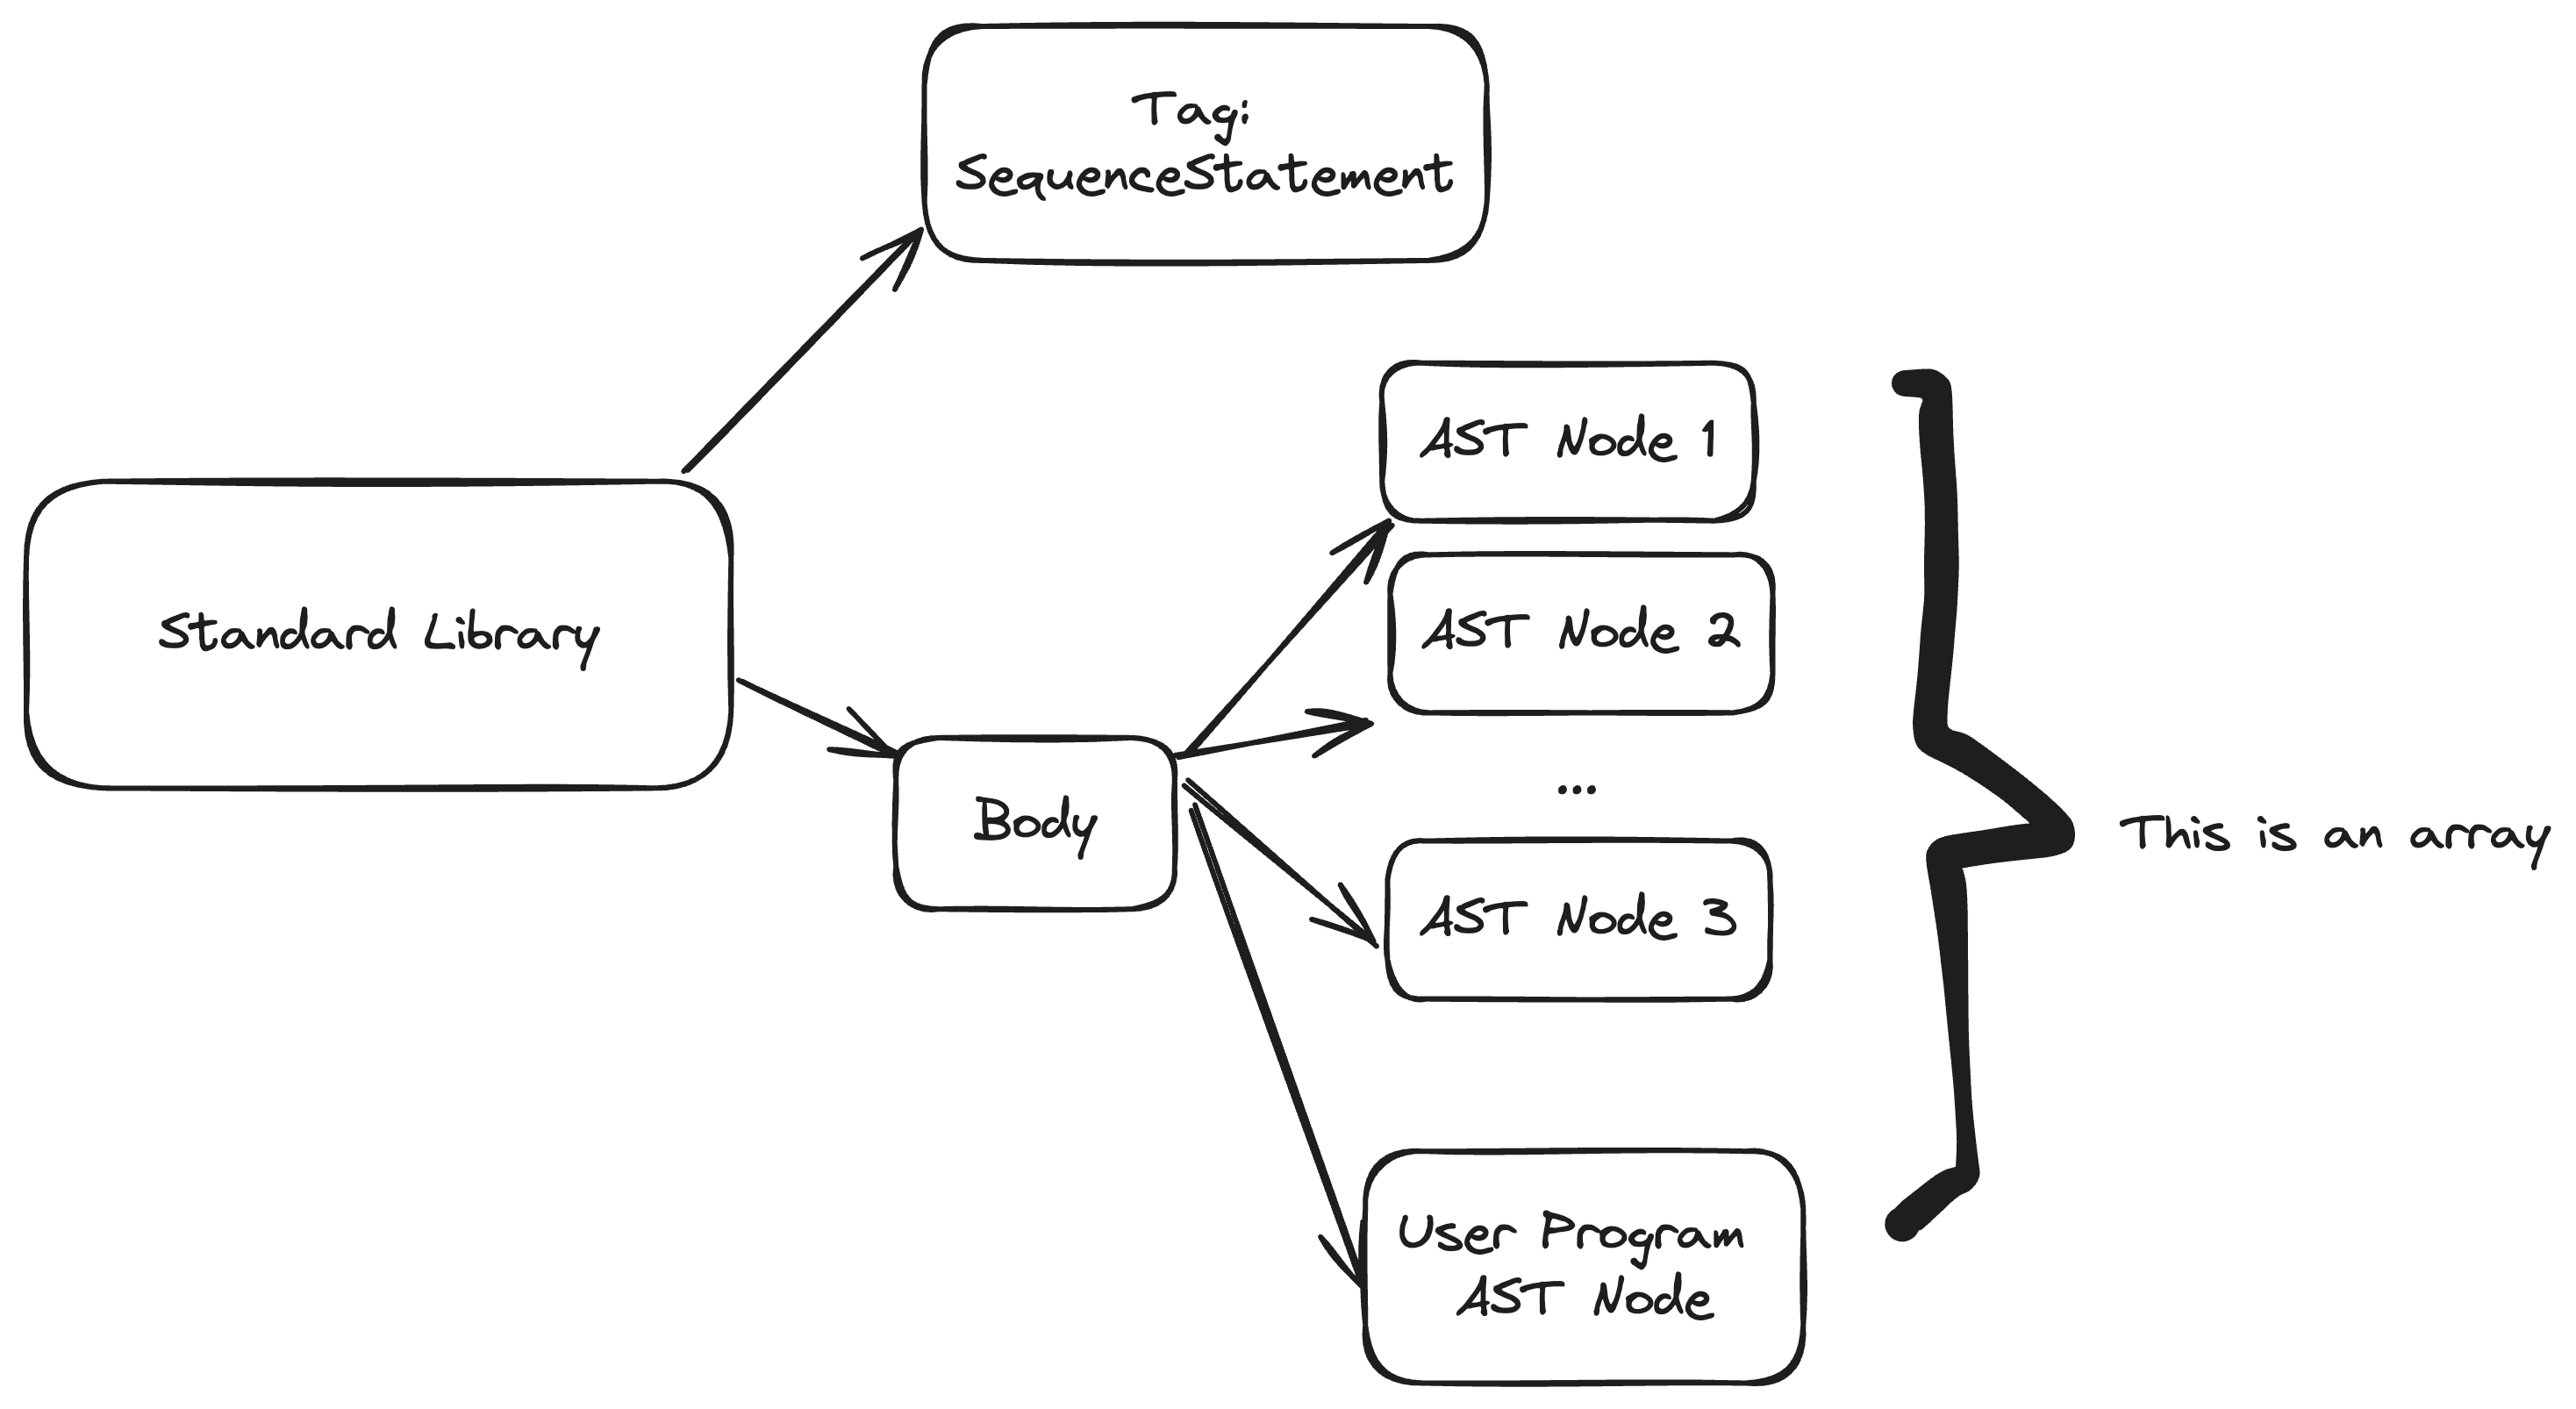
\includegraphics[width=0.75\textwidth]{images/AST-compilation.png}
    \caption{AST Compilation}
    \label{fig:ast-compilation}
\end{figure}

Finally, we wrap up the Standard Library AST node in its own block statement and compile the Standard Library AST node. Because the user program is a block that extends from the standard library's own block, the user can freely reference names from the standard library's frame while also being free to redefine standard library constructs, which provides ultimately flexibility for the developer.

At runtime, the VM will subsequently run through the standard library code, loading and assigning the expressions to their name bindings, before finally executing the user code. We chose to implement the standard library in addition to the builtin table so that we can easily handle custom structs such as Mutexes. Furthermore, because the BlockStatement produces a value and the user's program is the last element of the SequenceStatement, the return value of the program is the user's program return value. This allows us to test our programs easily by comparing the return value with an expected value.

\subsection{Concurrency Constructs}\label{section:concurrency}

Ooga supports the following concurrency constructs at the moment

\begin{enumerate}
    \item WaitGroups
    \item Mutexes
    \item Semaphores
    \item Buffered channels
    \item Unbuffered channels
    \item Select statement
\end{enumerate}

We first detail the thread scheduler that the Ooga VM runtime uses and how goroutines are spawned before diving into how the shared memory protection constructs are implemented.

\subsubsection{Thread Scheduler}

Ooga emulates Go's goroutines by employing the ThreadScheduler abstraction. The ThreadScheduler interface can be seen below

\begin{minted}{javascript}
export interface Scheduler {
    // ******* Supporting multiple executing threads

    // Get number of currently executing threads
    numCurrent(): number;
    // Get currently executing threads
    // list might be empty (none executing) or have more than 1 thread (parallelism?)
    currentThreads(): Iterator<ThreadId>;
    // Get number of idle threads
    numIdle(): number;
    // Get idle thread list
    idleThreads(): Iterator<ThreadId>;
    // Register a new thread into the scheduler (thread has never run before)
    // Returns the thread id this new thread should be associated with
    newThread(): ThreadId;
    // Unregister a thread from the scheduler (end of life/killed)
    // Thread should be currently executing
    deleteCurrentThread(id: ThreadId): void;
    // Get which thread should be executed next, and for how long
    // null means there are no idle threads to run
    runThread(): [ThreadId, number];
    // Tell scheduler which thread should be paused and placed back into the idle threads.
    pauseThread(id: ThreadId): void;
    // get the max time quanta, useful when a single thread only
    getMaxTimeQuanta(): number;
}
\end{minted}

For simplicity, we employ the Round Robin thread scheduler which maintains a set of active threads and a set of idle threads. It simply iterates through the list of threads in a round robin manner, and ensures that all threads are fairly distributed "CPU time".

Each thread is given a random number of instructions which it can execute for, known as its TimeQuanta. Upon reaching a TimeQuanta of 0, the thread times out and asks the ThreadScheduler to set up the next thread. This can be seen in a snippet of our VM code

\begin{minted}{javascript}
function runInstruction() {
    const instr = instrs[PC++];
    microcode[instr.tag](instr);
    if (blockedThreadState) {
        blockedThreadState = false;
        blockThread();
    }
    if (yieldThreadState) {
        yieldThreadState = false;
        timeoutThread();
    }
    if (!isAtomicSection) {
        TimeQuanta--;
    }
}

export function run(numWords = 1000000) {
    // initializes the VM with number of words
    initialize(numWords);
    while (running) {
        if (TimeQuanta > 0) {
            runInstruction();
        } else if (TimeQuanta === 0) {
            timeoutThread();
        } else {
            throw Error('TimeQuanta cannot be negative. \
                Something has gone horribly wrong.');
        }
        // Handle errors
        if (State !== ProgramState.NORMAL) {
            throw Error('execution aborted due to: ' + getErrorType());
        }
    }
    const returnValue = addressToTSValue(peekStack(OS[0]));
    return returnValue;
}    
\end{minted}

\subsubsection{Thread State and Shared Memory}

Each thread maintains its own independent copy of its E, OS, RTS and PC which reference the same javascript ByteArray shared among all threads. Ooga is thus able to replicate data races and race conditions because although each thread maintains its own E and OS, their E and OS may reference objects on the heap that are referenced to by other threads. We are thus able to replicate the classical read and write race conditions in Ooga programs.

A side tangent here into garbage collection: when GC is triggered, each thread pushes its E, OS and RTS into temporary roots that are marked as alive and subsequently forwarded. This ensures that a thread does not refer to garbage collected addresses which can corrupt the program's correctness.

When we change threads, we suspend execution of the current thread and save the current thread's E, RTS, PC and OS into an internal mapping from ThreadID to ThreadState. We then resume execution of the incoming thread after loading the incoming thread's E, RTS, PC and OS. This effectively achieves \textbf{context switching}. 

\subsubsection{Goroutines}

In Ooga, we spawn threads through the use of goroutines, similarly to Go. Ooga supports both goroutines on anonymous expressions, named functions and struct methods as seen below:

\begin{minted}{go}
// launch a goroutine on an anonymous function
a := 0;
go func() {
    a = a + 1;
}();

func foo() int {
    return a + 1;
}
// launch goroutine on named function
go foo();

type Vector struct {
    x int
    y int
}

func (v *Vector) Add(dx int, dy int) {
    v.x = v.x + dx;
    v.y = v.y + dy;
}

go v.Add(1, 1);
\end{minted}

Goroutines statements are supported in the parser as follows:

\begin{minted}{javascript}
GoroutineStatement
  = GoroutineToken _ argument:GoroutineCallExpression EOS {
      return { tag: "CallGoroutine", expression: argument }
    }

GoroutineCallExpression
  = head:(
      callee:MemberExpression __ args:Arguments { 
      // Handles function/method calls
        return { tag: "GoroutineCallExpression", callee: callee, arguments: args };
      }
    )
    tail:(
        // For additional method calls or property 
        // accesses after the initial call
        __ args:Arguments {
          return { tag: "GoroutineCallExpression", arguments: args };
        }
      / __ "." __ property:Identifier __ args:Arguments { 
        // Direct support for method calls with dot syntax
          return {
            tag: "GoroutineCallExpression",
            callee: {
              tag: "MemberExpression",
              object: head,
              property: property
            },
            arguments: args
          };
        }
    )*
    {
      return tail.reduce(function(result, element) {
        // Similar logic as CallExpression, adjusting 
        // based on whether it's a further 
        // call or property access
        if (element.tag === "GoroutineCallExpression" || element.tag === "CallExpression") {
          element.callee = result;
        } else { // For member expressions
          element.object = result;
        }
        return element;
      }, head);
    }
\end{minted}

At compilation time, we compile the function call expression as normal and then push a NEW\_THREAD and DONE instruction. The NEW\_THREAD instruction expects a closure on the OS stack when it is encountered along with the expected number of arguments which is handled natively by the compilation of the function expression. 

At runtime, when the VM encounters a NEW\_THREAD instruction, it first pops off the closure and then initializes a brand new OS, RTS and E by allocating onto the heap and setting the new thread's PC to the starting address of the closure. We then prepare the machine for a regular function call with respect to the new OS, RTS and E. The difference between this and a regular function call is that we also create a new thread using the scheduler, increment the PC of the current thread to step past the DONE instruction from the compiler, and then timeout the current thread. This means that the newly spawned goroutine immediately executes for its share of the CPU time. When the goroutine is done with the function computation, it returns to the closure and encounters the DONE instruction, whereupon it is killed off by the thread scheduler. Finally, on the thread which spawned the goroutine, we push TRUE onto the OS as all statements are expected to produce a value. This means that the goroutine expression does not push a closure onto the OS as we do with function declarations.

To be consistent with Go's specifications, when the main thread itself reaches a DONE instruction, the VM terminates the entire program execution regardless of the status of the other goroutines.

\subsubsection{Mutexes}

Mutexes are implemented in the standard library itself as follows:

\begin{minted}{go}
type Mutex struct {
    currentThread int
}

func NewMutex() Mutex {
    m := Mutex{-1};
    return m;
}

func (m *Mutex) Lock() {
    for {
        startAtomic();
        id := m.currentThread;
        if (id == -1) {
            break; // finally pick up lock
        }
        // else
        endAtomic();
        blockThread(); // block and loop until can pick up lock
    }
    m.currentThread = getThreadID();
    endAtomic();
}

func (m *Mutex) Unlock() {
    startAtomic();
    if m.currentThread == getThreadID() {
        m.currentThread = -1;
    } else {
        oogaError(); // custom error since we don't currently support returning errors
    }
    endAtomic();
}
\end{minted}

Users would instantiate mutexes using the NewMutex() function and call Lock and Unlock accordingly. The builtin functions startAtomic, endAtomic, blockThread, oogaError and getThreadID are introduced here to facilitate the implementation of the mutex.

The startAtomic and endAtomic instructions simply stop the TimeQuanta from decrementing when an instruction is run, thereby emulating "atomicity". The blockThread is similar to yieldThread except that it signals to the VM that the current thread is blocked, which is used for our \textbf{naive deadlock detection} wherein we terminate the program early if we detect that all threads are currently blocked after one round robin across all threads. getThreadID returns the current thread ID and is used to enforce that only a single thread can acquire the mutex and subsequently release it. We are thus able to support the standard mutexes as taught in concurrency 101.

A limitation of our current approach is that we do not have encapsulation and are therefore unable to prevent the user from instantiating a mutex themselves and passing in a currentThreadId other than -1, which breaks the implementation.

A possible future extension we would thus do is to emulate Golang's use of lower and upper case identifier to distinguish between a public and a private name. At compilation time, we note whether a name is public or private when declaring a name. At name look up time, we simply check if the name look up is in the current frame, if so, the look up always succeeds. If not and the name is private, the look up fails. Due to time constraints, we will not be implementing this but it remains a possible stretch goal for the future.

\subsubsection{Semaphores}

Semaphores are also implemented in the standard library itself as follows:

\begin{minted}{go}
type Semaphore struct {
    count int
}

func (s *Sync) NewSemaphore(count int) Semaphore {
    s := Semaphore{count};
    return s;
}

func (s *Semaphore) Down() {
    for {
        startAtomic();
        if (s.count > 0) {
            s.count = s.count - 1;
            break;
        }
        endAtomic();
        blockThread();
    }
    endAtomic();
}

func (s *Semaphore) Up() {
    startAtomic();
    s.count = s.count + 1;
    endAtomic();
}    
\end{minted}

Semaphores are given a similar treatment to mutexes, except that we follow the formalism provided in the lecture notes on concurrency, wherein semaphores do not explicitly wake up other sleeping threads when Semaphore::Up() is called.

We now take a side tangent to discuss the design choices of mutexes and semaphores. We had originally planned to make mutexes and semaphores separate nodes that lived on the heap with their own Tags and interfacing functions which were treated specially by the oogavm-machine source code. This would have allowed us to make use of Javascript Map objects to map the thread dependencies on the mutexes and semaphores to come up with more sophisticated deadlock detection schemes compared to our current naive implementation. We ultimately chose to implement mutexes and semaphores using the standard library itself due to the simplicity and to demonstrate the expressiveness of our custom language (and standard library) in implementing classical constructs. Future work would likely integrate the mutexes and semaphores into the interpreting language (Javascript) itself.

\subsubsection{WaitGroups}

WaitGroups are implemented entirely in the standard library elegantly and simply as follows:

\begin{minted}{go}
type WaitGroup struct {
    counter int
}

func (s *Sync) NewWaitGroup(counter int) WaitGroup {
    wg := WaitGroup{counter};
    return wg;
}

func (wg *WaitGroup) Add(delta int) {
    startAtomic();
    wg.counter += delta
    endAtomic();
}

func (wg *WaitGroup) Done() {
    // update expressions are atomic
    wg.counter--
}

func (wg *WaitGroup) Wait() {
    for {
        startAtomic();
        if wg.counter <= 0 {
            endAtomic();
            break;
        }
        endAtomic();
        yieldThread(); // yield to avoid wasteful loop
    }
}
\end{minted}

The WaitGroup maintains an internal counter and then waits on the counter to drop to 0 before terminating function control. At each iteration, we call the builtin function yieldThread which sends a signal to the VM to time out the thread thereby avoiding wasting CPU time on redundant computation since our single threaded javascript runtime clearly cannot progress the other goroutines. All updates and checks are done atomically.


\subsubsection{Buffered and unbuffered channels} \label{section:channels}

Channels are handled by the parser as follows

\begin{minted}{javascript}
CallExpression
    = ...
    / MakeToken __ "(" __ type:InitType __
    \ args:MakeArguments? __ ")" {
        return {
            tag: "MakeCallExpression",
            type: type,
            args: args || []
        };

MakeArguments
  = "," __ args:ArgumentList {
      return args
    }

ChannelReadExpression
    = "<-" __ channel:Expression {
      return {
        tag: "ChannelReadExpression",
        channel: channel
      };
    }

ChannelWriteExpression
    = channel:Expression __ "<-" __ value:Expression EOS? {
        return {
            tag: "ChannelWriteExpression",
            channel: channel,
            value: value
        };
        }
\end{minted}

At parser time, we populate the AST node with whether it is a Channel or Slice type. At compilation time, we create a buffered or unbuffered channel depending on whether a number was passed to the make call as the second argument, similar to Go. Thus Ooga supports the following expressions

\begin{minted}{go}
a := make(chan int); // unbuffered channel
b := make(chan bool, 1); // buffered channel of size 1
c := make(chan Struct, 5); // buffered channel of size 5

go func() {
    a<- 5; // write to unbuffered channel
}
d := <-a; // read from unbuffered channel
b<- 5; // write to buffered channel
\end{minted}

Our treatment of buffered and unbuffered channels strictly follow Go's treatment. Read and writes to an unbuffered channel block unless there is a corresponding write and read from that same unbuffered channel. Reading from a buffered channel blocks if the buffered channel is empty and writing to a buffered channel blocks if it is full, the operation is non blocking in every other case. 

At compilation time, we first compile the value (if it's a write) and then the channel component (for both read and writes). As we do not have information about the type of channel, we simply push the machine instruction READ\_CHANNEL for ChannelReadExpressions and WRITE\_CHANNEL and CHECK\_CHANNEL for ChannelWriteExpressions that are handled at runtime.

Now we detail the different operations at runtime, detailing the simpler read operation first. 

When reading, we first pop the channel from the OS and determine its type. Regardless of its type, we block if the channel is empty and consume the value if it is not.

Writing to a channel is more complicated and necessitates the use of the CHECK\_CHANNEL operation. We first perform the WRITE\_CHANNEL which pops a channel and the value to write from the OS. In both cases, the WRITE\_CHANNEL pushes the channel onto the OS after completion so that the CHECK\_CHANNEL can read the same channel.

\textbf{Case 1: Unbuffered channel}. If the channel is full, we simply decrement the PC (so that we will repeat the instruction), push the channel and value onto the OS and then call the builtin blockThread call. Eventually, we will be able to push the value onto the unbuffered channel in the absence of a deadlock. We now navigate to the CHECK\_CHANNEL instruction. Because we can only unblock from the write when the value is consumed, we do the same trick earlier, we block if the channel is not empty and only unblock when the channel is empty as this indicates that a thread has consumed the unbuffered channel. In the event that the value is never consumed, we effectively starve the thread. This thus corresponds to how Golang performs an unbuffered channel.

\textbf{Case 2: Buffered channel}. This is the simpler case. We block until we are eventually able to push the value onto a non-full channel. This can result in a starved thread if no other threads consume a value. At CHECK\_CHANNEL, we consume the channel and stop.

We have now shown that we have effectively emulated the language specifications of Golang channels and now proceed to detail the final concurrency feature of Golang, select statements.

\subsubsection{Select Statements}

Ooga is a partially faithful reproduction of Go's select statement. The select statement lets a goroutine wait on multiple communication operations and blocks until one of its cases can run then it executes that case. In Go, if there are more than one available cases, it is chosen at random. In Ooga however, we check each case sequentially and execute the first case that is available, we thus do not have random execution.

Select statements support the following 4 kinds of expressions: a channel read operation with an assignment, a channel read expression without an assignment, a channel write expression and a default case.

\begin{minted}{go}
select {
     case i := <-c:
         fmt.Printf("Received %d\n", i)
     case c <- 0:
         fmt.Println("Sent 0")
     case <-quit:
         fmt.Println("Quit")
     default:
         fmt.Println("No communication")
}
\end{minted}

These are handled by the peggy parser as 

\begin{minted}{javascript}
SelectClause
  = CaseToken __ varDecl:ChannelVariableStatement __ ":" __ body:(__ StatementList)? __ {
    return {
      tag: "SelectReadVariableCase",
      operation: varDecl,
      body: {tag: "BlockStatement", body: optionalList(extractOptional(body, 1))}
    };
  }
  / CaseToken __ chanop:ChannelReadExpression __ ":" __ body:(__ StatementList)? __ {
    return {
      tag: "SelectReadCase",
      operation: chanop,
      body: {tag: "BlockStatement", body: optionalList(extractOptional(body, 1))}
    };
  }
  / CaseToken __ chanop:ChannelWriteExpression __ ":" __ body:(__ StatementList)? __ {
    return {
      tag: "SelectWriteCase",
      operation: chanop,
      body: {tag: "BlockStatement", body: optionalList(extractOptional(body, 1))}
    };
  }

SelectDefaultClause
  = DefaultToken __ ":" __ body:(__ StatementList)? __ {
    return {
      tag: "SelectDefaultCase",
      body: {tag: "BlockStatement", body: optionalList(extractOptional(body, 1))}
    };
  }
\end{minted}

The Select statement is handled very similarly to the Switch statement with jumps placed at the end of every case to support the implicit break. The only difference now is that we must be able to attempt a read or a write to the channel without blocking the thread, only blocking if none of the cases match. In the presence of a default case, the select never blocks.

To support reading and writing to channels without blocking, we introduce two new machine instructions CHECK\_READ and CHECK\_WRITE which merely push True if the channel can be read from or written to and False otherwise. For each Select case expression, we push the appropriate CHECK instruction followed by a JOF machine instruction that jumps to the next case, just like how Switch is handled. If the JOF does not jump, we then either read or write to the channel.

This entire operation must be wrapped up in an atomicity block of START\_ATOMIC and END\_ATOMIC because it is possible that a thread checks that a channel can be operated on, pushes True, then gets context switched and another thread pushes or reads from that same channel, violating the invariant that the channel is safe to operate on. The atomicity block wrapping prevents the thread from getting context switched.

To make the select statement block in the absence of a default case, a BLOCK\_THREAD instruction is pushed at the end of the cases if a default case was not encountered, followed by a GOTO instruction to the beginning of the select case, to simulate the fact that the select case will block until a channel can be operated on. In every other aspect, the select case is thus fundamentally equivalent to the switch case.

\section{User Interface}

Our frontend interface serves as the central point of interaction for users working with our Ooga system. This interface provides a development environment for writing, executing, and debugging Ooga code, and is fully integrated with our backend services. This enables real-time execution and debugging capabilities that are crucial for effective development in the Ooga programming language.

\subsection{Server Architecture}

The backend server is an integral component of our system's functionality, developed using the Express.js framework. It provides a RESTful API that facilitates communication between the frontend and the Ooga virtual machine. When users submit their code through the frontend interface, the server processes this code, executes it using the Ooga VM, and captures any resultant output. This output could include standard program output, errors, or system warnings, which are then relayed back to the user through the frontend interface.

In addition to execution, the backend is designed to handle debugging operations. When a user sets breakpoints within their code—marked by \texttt{breakpoint} statements, the server captures and sends detailed runtime state information to the frontend. This information includes the operand stack (OS) and run-time stack (RTS) of each thread, as well as a snapshot of the heap at the moment the breakpoint is hit.

\subsection{Frontend Structure}

The frontend of the Ooga system, built with React, primarily features two Monaco editors; one serves as the code editor, and the other displays the program's output, including any runtime messages or errors. This dual-editor setup is illustrated in Figure \ref{fig:editor-view}.

\begin{figure}
    \centering
    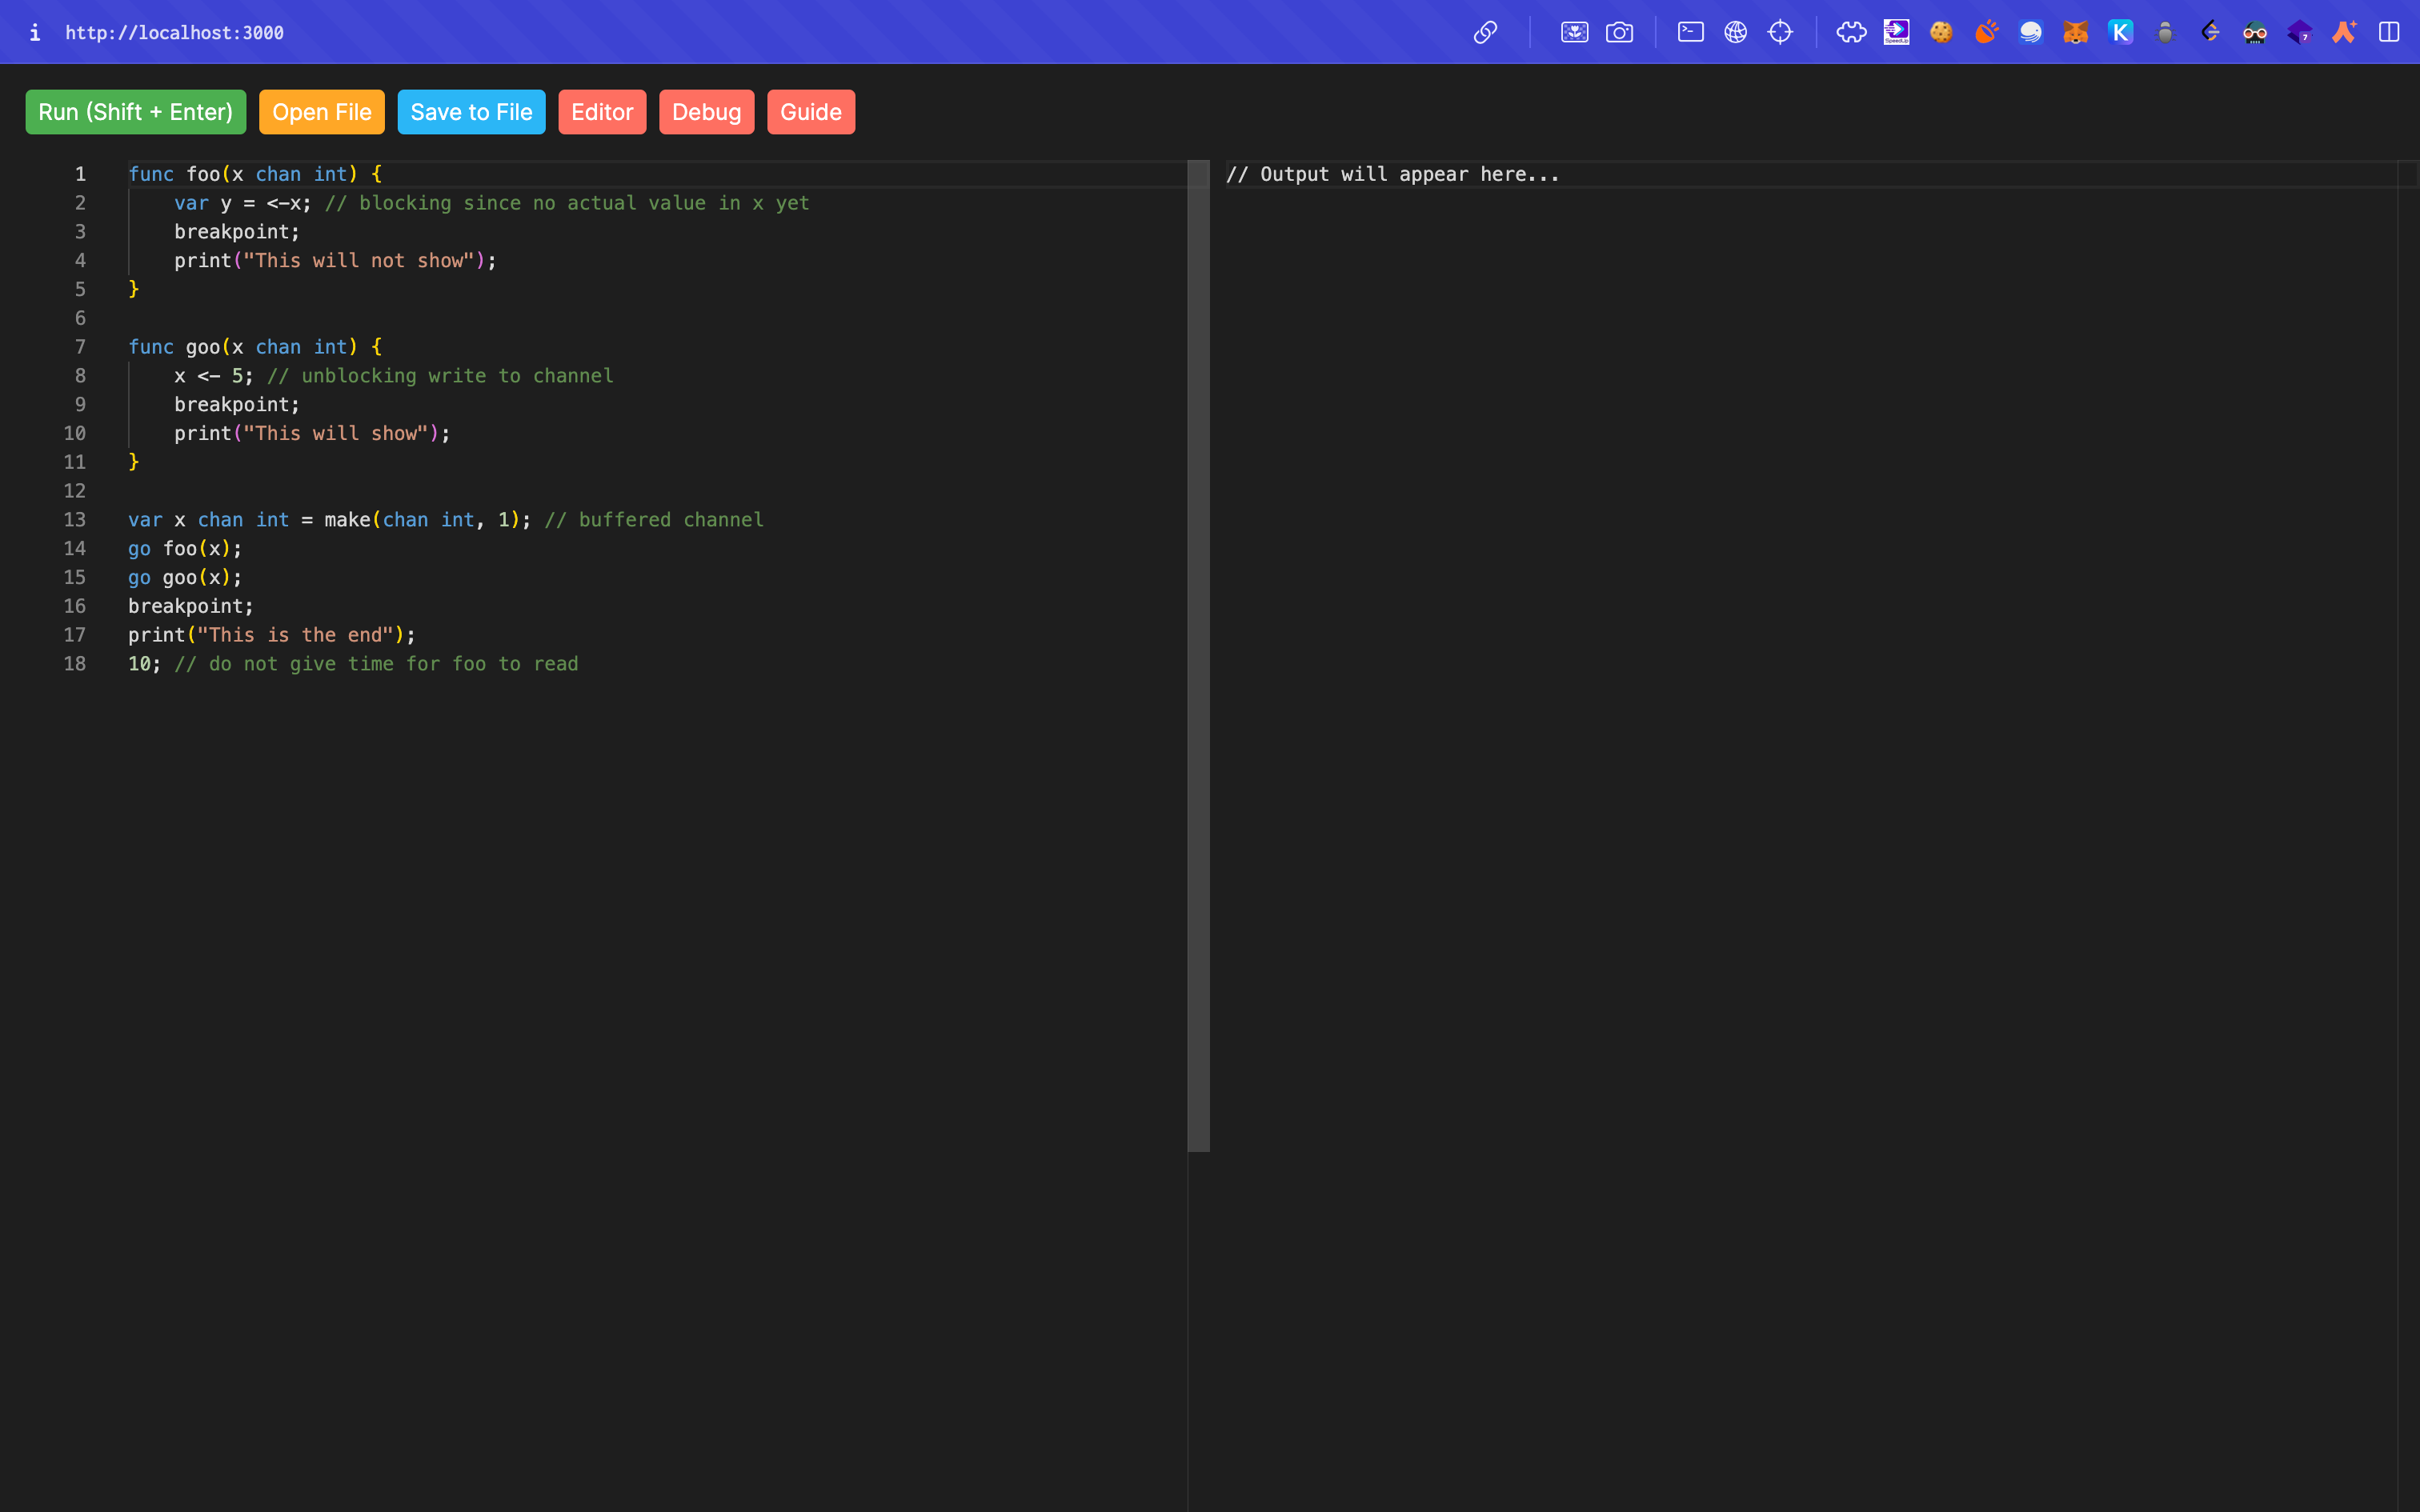
\includegraphics[width=1.0\linewidth]{images/editorview.png}
    \caption{The primary editor interface, showing both code input and output panels.}
    \label{fig:editor-view}
\end{figure}

A core element of the frontend is the debug view, which leverages the ReactFlow library to visualize the operational stack (OS) and run-time stack (RTS) of all active threads, as well as the heap states captured by the server upon encountering \texttt{breakpoint} statements. Each frame within these stacks is represented as a node within a flowchart, connected by edges that show their linkage. Custom nodes are used to display pertinent information such as memory addresses, values stored at those addresses, and other metadata.

\subsection{Debugging and Visualization Enhancements}

Enhancing the debugging experience is a focal point of our development efforts. We incorporate comprehensive visualization tools that help the user debug their programs by providing intuitive and interactive representations of the program's runtime state at specified breakpoints.

\textbf{Stack Visualization:}
The \texttt{StackView} component provides a graphical depiction of the OS and RTS stacks associated with each thread. This visualization is interactive, allowing users to select and inspect individual stack frames for detailed information like memory addresses and their contents. Below is a code snippet that illustrates how stack data is dynamically converted into visual elements:

\begin{minted}{typescript}
// Component to visualize thread stacks using ReactFlow
function StackView({ data, currentThreadIndex }) {
  const [nodes, setNodes] = useState([]);
  const [edges, setEdges] = useState([]);

  useEffect(() => {
    let localNodes = [];
    let localEdges = [];

    // Populate nodes and edges for each thread's stack
    data.forEach((threadData, index) => {
      const { nodes: threadNodes, edges: threadEdges } = createNodesAndEdges(
        threadData,
        index * 600,
        index,
        index === currentThreadIndex
      );
      localNodes = [...localNodes, ...threadNodes];
      localEdges = [...localEdges, ...threadEdges];
    });

    setNodes(localNodes);
    setEdges(localEdges);
  }, [data, currentThreadIndex]);

  // Additional component logic...
}
\end{minted}

The thread that the breakpoint statement was triggered from is highlighted in yellow, which could also assist the user in understanding which breakpoint it is referring to.

\textbf{Heap Visualization:}
Similarly, the \texttt{HeapView} component illustrates the heap's state using nodes and edges to represent objects and their relationships (such as parent-child links). Users can interact with this graph to uncover details about each object, including its memory address, size, type (tag), and the values it holds. This feature is particularly valuable for understanding complex memory layouts and diagnosing memory-related issues. The user can also click on nodes in this graph, which highlights not only the node itself (blue) but also its parents (red) and children (green) recursively. The heap and stack view can be seen in Figure \ref{fig:stack-heap-view}.

\begin{figure}
    \centering
    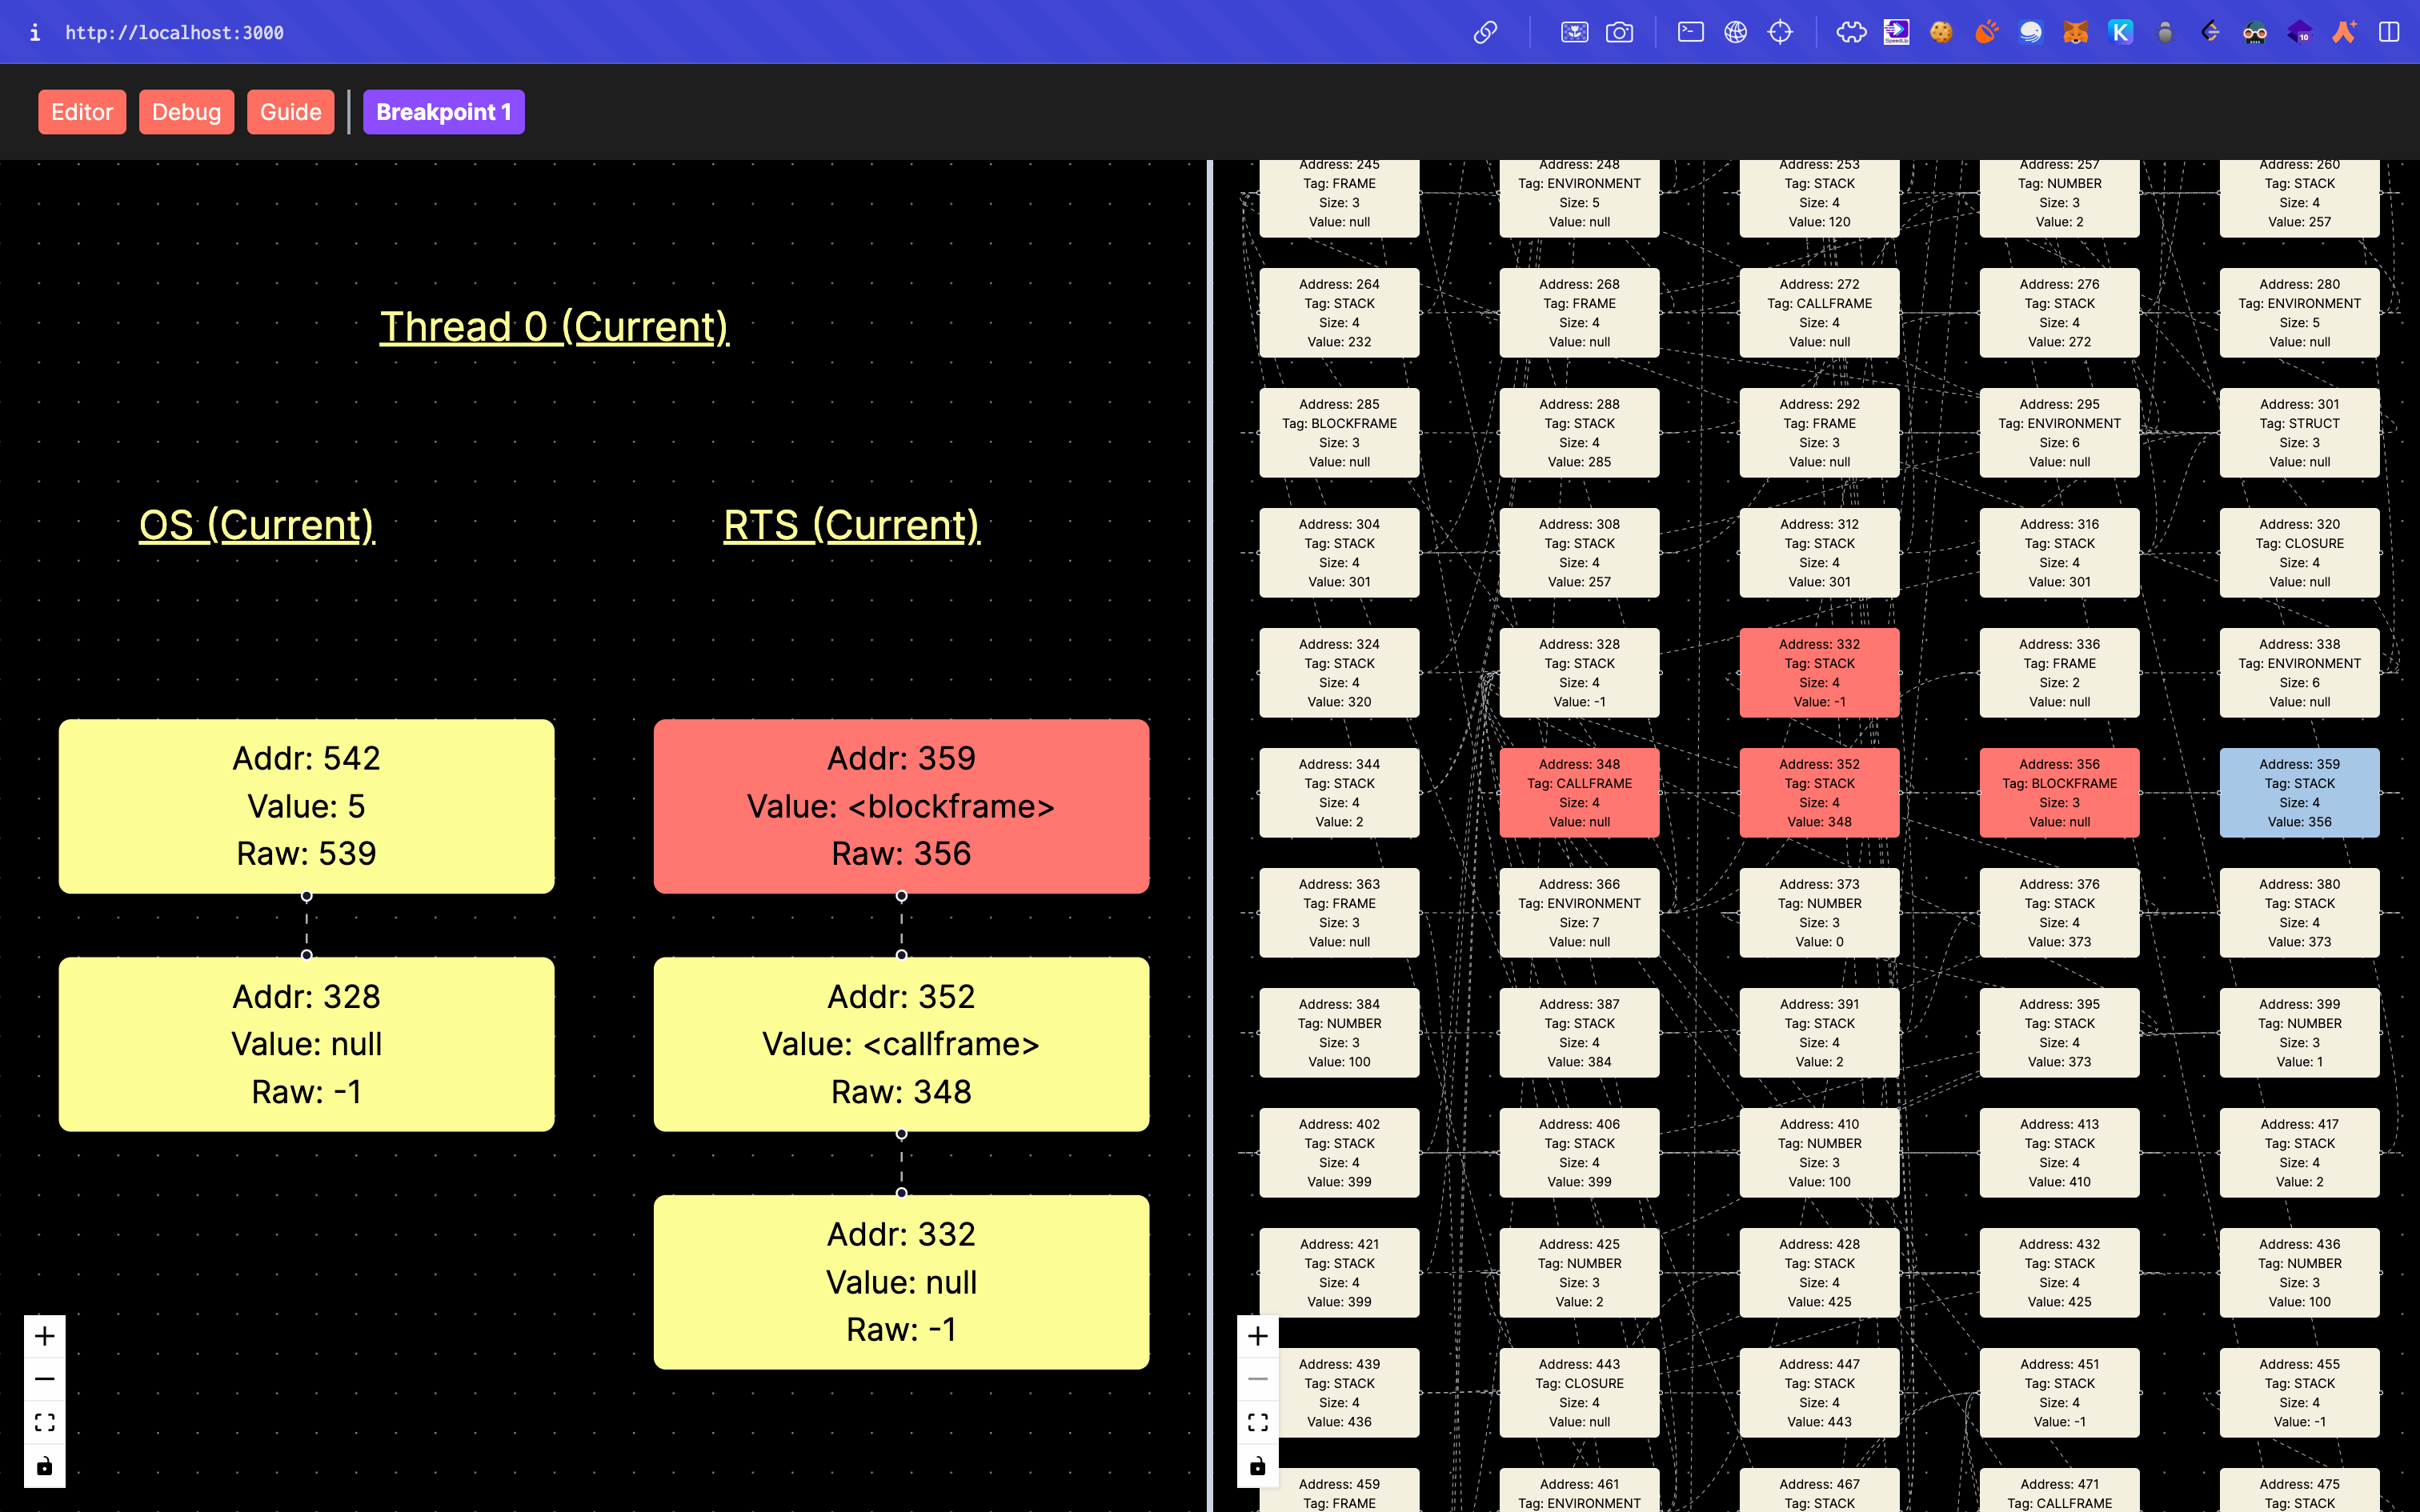
\includegraphics[width=1\linewidth]{images/stackheapview.png}
    \caption{Visualization of both stack and heap states during a debug session.}
    \label{fig:stack-heap-view}
\end{figure}

\textbf{Breakpoint Functionality:}
Our system’s debugging capabilities are significantly enhanced by the use of breakpoints. When a breakpoint is reached during execution, the system captures and displays the state of all threads and the heap at that moment. This feature allows developers to inspect the state of the program at critical points, letting them get a deeper understanding of the execution flow and quickly identifying errors.

The integration of these debugging and visualization tools into the Ooga development environment empowers our users to write, execute, and debug their programs efficiently. 

\subsection{User Guide}

\begin{figure}
    \centering
    \includegraphics[width=1\linewidth]{images/userguide.png}
    \caption{User Guide}
    \label{fig:user-guide}
\end{figure}

We also provide a user guide on our frontend itself, which should help the user get started quickly with coding in Ooga and in using our editor and debugger effectively. This can be seen in Figure \ref{fig:user-guide}.

\section{Running Ooga}

The Ooga language repository can be found at \url{https://github.com/CS4215-OOGA/Ooga} while the frontend can be found at \url{https://github.com/CS4215-OOGA/ooga-frontend}. The README in the repository contains detailed instructions for setting up and running the project but the instructions are repeated here for brevity.

The language server is easy to set up. Simply run \texttt{yarn install} to install all the necessary packages, then \texttt{yarn peggy} to generate the grammar javascript file using peggy, and lastly \texttt{yarn server} to build the entire project and run the server that the frontend uses for communication. The default port used for this is 3001, but you may change it in \texttt{src/server/server.ts}.

For additional debug messages, run \texttt{export DEBUG=*} before running the above commands.

To run the frontend locally, simply run \texttt{npm install} to install necessary packages, then either \texttt{npm run dev} for a developer version with hot reloading etc. This frontend will be accessible on \url{http://localhost:3000}.

\section{Test Cases} \label{section:test-cases}
Our comprehensive test suite evaluates a wide array of scenarios to ensure robustness and correctness across all features of the Ooga language. This section highlights some key test cases that demonstrate the capabilities and edge cases of our implementation.

We begin by briefly explaining how our testing suite is implemented. 

\begin{minted}{javascript}
export function testProgram(
    program: string,
    expectedValue: any,
    expectedOutput: string,
    numWords: number = defaultNumWords
) {
    // Prepare debug logs
    ...
    try {
        // Prepare, run and capture return value 
        // and output from program
        ...
    } catch (e) {
        // If error is intended error, success. (Negative testing)
        ...
    } finally {
        debug.enable('*');
    }

    if (value !== expectedValue) {
        // Print expected value versus actual value
        ...
    } else if (capturedOutput.trim() !== expectedOutput?.trim()) {
        // Print expected output versus actual output
        ...
    } else {
        logTest('Test passed');
        logTest('--------------------------------------------');
    }
}    
\end{minted}

Our test suite captures the standard output of the user program as well as the return value. This allows us to use print statements to automatically verify the control flow of programs. We also support negative testing, to check that our compiler and VM successfully catch intentional errors. Finally, we support the testing of our Garbage Collection by passing in a custom number of words for the heap size.

\subsection{Sequential Language Constructs}

The following test case demonstrates our simple, sequential language constructs.

\begin{minted}{go}
var x int = 5; // manual type declaration
x; // returns 5

y := 5; // automatic type inference
y; // returns 5

const z int = 10;
// z = 11; // will throw an error

{
    // demonstrates block scoping
    var z = 11;
    x = 6;
    print(z); // will print 11
    print(x); // will print 6
}

print(z); // will print 10
print(x); // will still print 6

// Test that lambda expressions are supported
foo := func(n int) int {
    return n;
};
foo(5); // returns 5
\end{minted}

\begin{minted}{go}
// Demonstrates default initialization
type Vector struct {
    x int
    y int
    z Vector
}

var x int; // defaults to 0
print(x); // 0

var y bool;
print(y); // false

var z string;
print(z); // ""

var a Vector;
var b Vector = Vector{1, 2, Vector{3, 4, nil} };

print(a.x); // 0
print(a.y); // 0
print(a.z); // "nil"

print(b.x); // 1
print(b.y); // 2
print(b.z); // "<struct>"

print(nil); // "nil"
print(a.z == nil); // true
\end{minted}

\begin{minted}{go}
// Test struct methods
type Point struct {
    x int;
    y int;
}

func (p Point) getX() int {
    return p.x;
}

func (p Point) addX(n int) int {
    return p.x + n;
}

var p Point = Point{1, 2};

p.addX(5);
\end{minted}

\subsection{Control Flow}

The following tests demonstrate our control flow constructs.

\begin{minted}{go}
var x int = 5;
if (x == 5) {
  6;
} else {
  7;
} // the return value is 6 as explained earlier
\end{minted}

\begin{minted}{go}
var x int = 6;
if (x == 5) {
  6;
} else {
  7;
} // the return value is 7 as explained earlier
\end{minted}

\begin{minted}{go}
// Tests classical recursive function calls
func factorial(n int) int {
  if (n == 1) {
    return 1;
  } else {
    return n * factorial(n-1);
  }
}
factorial(5); // returns 120
\end{minted}

\begin{minted}{go}
// Tests for loop with init, test and update using var
var sum int = 0;
for var i int = 0; i < 10; i = i + 1 {
  sum = sum + i; // returns 45
}
\end{minted}

\begin{minted}{go}
// Tests for loop with init, test and update using short hand
var sum int = 0;
for i := 0; i < 10; i = i + 1 {
  sum = sum + i; // returns 45
}   
\end{minted}

\begin{minted}{go}
// Tests for loop with only condition
var i int= 0;
for i < 10 {
  sum = sum + i; // returns 45
  i = i + 1; 
}   
\end{minted}

\begin{minted}{go}
// Tests infinite loop with break
var sum int = 0;
var i int = 0;
for {
  if (i == 10) {
    break;
  }
  sum = sum + i; // returns 45
  i = i + 1;
}   
\end{minted}{go}

\begin{minted}{go}
// Test nested for loops
var sum int = 0;
for var i int = 0; i < 10; i = i + 1 {
  for j := 0; j < 10; j++ {
    sum = sum + i + j; // returns 900
  }
}
\end{minted}

\begin{minted}{go}
// Tests continue
var sum int = 0;
for var i int = 0; i < 10; i = i + 1 {
  if (i == 5) {
    continue;
  }
  sum = sum + i;
}   
\end{minted}

\begin{minted}{go}
// Tests higher order functions
func foo(f func(int) int) int {
    return f(5);
}

func goo(x int) int {
    return x + 5;
}

foo(goo); // returns 10
\end{minted}


\subsection{Type Checker}

The first demonstrates the type checker's assertions:
\begin{minted}{go}
type Vertex struct {
x int
y int
}

// Various ways of 
var a = Vertex{1,2}
b := Vertex{x: 1, y: 2}
var c Vertex = Vertex{1,2}

// Error due to type mismatch between user-declared type and initialization type
var d int = Vertex{2,3}

var e int = 5
// Error due to assignment type mismatch: expected int, got string
e = "hello"

const f int = 10
// Error due to constant reassignment
f = 6
\end{minted}

\subsection{Standard Library}

The next test case showcases our standard library functions, such as the presence of mutexes, semaphores, fmt and sleep implementations:

\begin{minted}{go}
// Show the standard library
m := sync.NewMutex();
s := sync.NewSemaphore(2);
fmt.Println("The magic number is: " + 5);
time.Sleep(1000); // sleep for 1000 milliseconds, or 1 second
// Stdout:
// "The magic number is: 5"
\end{minted}

\subsection{Concurrency}

Next we showcase basic concurrency patterns. We first demonstrate goroutines and WaitGroups. The first goroutine has a much longer for loop runtime than the second, hence the second goroutine's print happens first and we expect the output \texttt{1} to be printed before \texttt{2}.

The WaitGroup is necessary as without it (especially the \texttt{wg.Wait()} statement at the end), the main thread and hence the whole program will finish running before either goroutine's print statement can execute, as per the Go language's runtime semantics. This test case also demonstrates our context switching between the various threads at play here.

\begin{minted}{go}
wg := sync.NewWaitGroup(2);

go func() {
    for i := 0; i < 100; i++ {

    }
    print("2");
    wg.Done();
}();

go func() {
    for i := 0; i < 10; i++ {

    }
    print("1");
    wg.Done();
}();

wg.Wait();
// Stdout:
// "1"
// "2"
\end{minted}

The next test evaluates the select statement implementation alongside the functionality of buffered and unbuffered channels, emphasizing the non-blocking and blocking behavior as specified in Section \ref{section:channels}. In this test case, x is declared with a capacity of 5 and is therefore a buffered channel. Each goroutine executes and pushes 1 onto the channel. When Select is executed, due to our partially faithful First Come First Serve implementation, the first case executes as we are able to perform a non-blocking read from X. The channel will subsequently be empty so the read would block, thus moving onto the next case where we are able to push 5 into the channel. At the fourth and final iteration, the first select case triggers again and 5 is printed.

\begin{minted}{go}
var x chan int = make(chan int, 5);

func foo() {
    x<- 1;
}

go foo();
go foo();

for i := 0; i < 4; i++ {
    select {
        case i := <-x:  // this will happen twice first, so print 1 twice, then finally print 5
            print(i);
        case x<- 5:     // finally this will happen and we will push 5 inside
            print(3);
        default:
            break;
    }
}

// in the end, print 1 1 3 5
10;
// Stdout:
// 1
// 1
// 3
// 5
// Program value: 10
\end{minted}

We now demonstrate the unbuffered channel. Although the fooga goroutine happens first, unbuffered channels are essentially buffered channels with capacity 0, and therefore a write blocks until there is a subsequent read. We therefore witness 0 being printed followed by "booga", 1 being printed, and finally "fooga". This test case demonstrates that our unbuffered channels work as expected. 

\begin{minted}{go}
func fooga(x chan int) {
    // writes to x, should block
    print(0);
    x <- 1;
    print("fooga"); // this should print after booga
}

func booga(x chan int) {
    var y int = <-x; // reads from x
    print("booga"); // this should print before fooga
    print(y); // check that 1 was received
}

var x chan int = make(chan int); // unbuffered channel
go fooga(x);
go booga(x);

for i := 0; i < 10; i++ {
    // do nothing to stall to see 'fooga' being printed
}
\end{minted}

We now show a select statement that blocks forever, and since the main thread exits so does the entire program. The two print statements never execute. This is because the channel \texttt{x} is never written to, and with the select statement being blocking (due to no eligible cases and no default), the following print statements do not run.

\begin{minted}{go}
x := make(chan int); // unbuffered

go func() {
    select {
    case <-x:
        print("This won't happen");
    }
    print("This also will not show");
}();

for i := 0; i < 100; i++ {
}
10;
// Program value: 10
\end{minted}

Next, we show our naive deadlock detection. When all running threads are deemed to be blocked, meaning that none can progress, we issue an error to the user, letting them know that their program is in such an undesired state.

\begin{minted}{go}
x := make(chan int); // unbuffered

select {
case <-x:
    print("This won't happen");
}
10;
// Error: Stuck forever!
\end{minted}

Now we demonstrate our mutexes. 3 goroutines are spawned which each try to mutate x by first acquiring the lock. The first goroutine that acquires the lock immediately yields, passing control to the main thread, which spawns the second goroutine. When the second goroutine fails to acquire the lock, it blocks and control is passed to the first goroutine (due to our round robin scheduler), which increments x and then unlocks the mutex. Control is passed to the second goroutine which finally acquires the lock and then yields to the main thread, spawning the final goroutine which blocks on the mutex and eventually increments x safely when the second goroutine is done. Thanks to the deterministic ordering of our round robin scheduler, we are able to fully reason out the ordering of simple concurrent programs to verify correctness of the mutex. This test case further demonstrates the correctness of our WaitGroup construct.

\begin{minted}{go}
var x int = 0;
wg := sync.NewWaitGroup(3);

func goo(i int, m Mutex) {
    print(i + " just started");
    m.Lock();
    print(i + " is locking");
    yieldThread(); // immediately give up again
    print(i + " is incrementing");
    x = x + 5;
    m.Unlock();
    wg.Done();
}

m := sync.NewMutex();

for i := 0; i < 3; i++ {
    go goo(i, m);
}

wg.Wait();
print(x);
\end{minted}

This test case on concurrency, uses a semaphore with 2 counts. The first 2 goroutines decrement the semaphore's count which blocks the third goroutine. When the main thread increments X and the semaphore, the third thread is able to proceed, thus resulting in our print order of 1,2 and 4.

\begin{minted}{go}
s := sync.NewSemaphore(2);
x := 0;

go func() {
    s.Down();
    x = x + 1;
    fmt.Println("x in Thread 1 is " + x); // this should be 1
}();

go func() {
    s.Down();
    x = x + 1;
    fmt.Println("x in Thread 2 is " + x); // this should be 2
}();

go func() {
    s.Down();
    x = x + 1;
    fmt.Println("x in Thread 3 is " + x); 
    // this should be 4 because main wakes up
    s.Up();
}();

x = x + 1;
s.Up();

for i := 0; i < 100; i++ {
}
\end{minted}

Our final test case demonstrates race conditions that can occur when concurrency protection constructs are not used (see Figure \ref{fig:race-condition}).

\begin{minted}{go}
x := 0;
wg := sync.NewWaitGroup(2);

func foo() {
    for i := 0; i < 1000; i++ {
        x = x + 1;
    }
    wg.Done();
}

go foo();
go foo();

wg.Wait();

print(x);
\end{minted}

In this classical example, we'd expect the final value of x to be 2000. Running the same program multiple times will demonstrate that this does not happen, due to the lack of synchronization over writing to shared memory, confirming that Ooga is able to replicate race conditions. The intelligent reader may use any such synchronization constructs such as mutexes, semaphores or even channels to produce a program that results in a final value of 2000 for x.

\begin{figure}
    \centering
    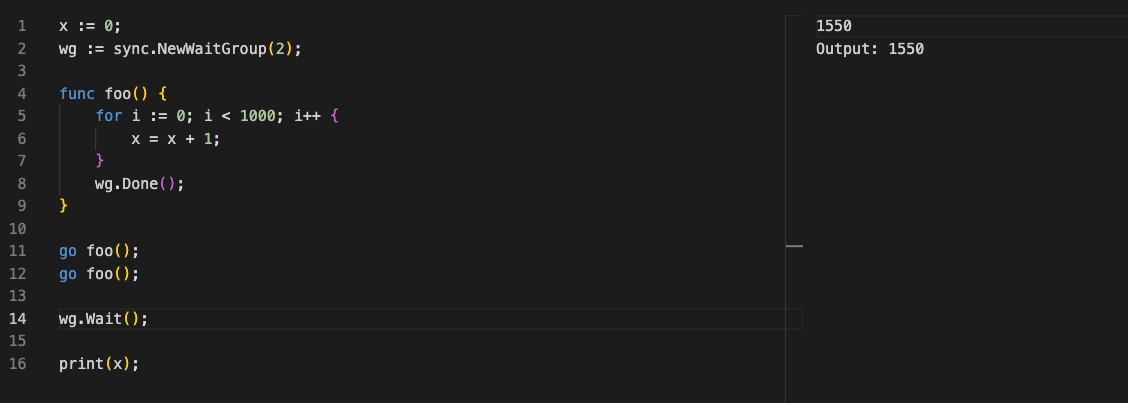
\includegraphics[width=\textwidth]{images/ooga-race-condition.png}
    \caption{Demonstration of race condition}
    \label{fig:race-condition}
\end{figure}

\subsection{Memory}

The next test case aims to show the variable node size, as opposed to the hardcoded 10-node limit the original in-class implementation had:
\begin{minted}{go}
var a int = 1;
var b int = 2;
var c int = 3;
var d int = 4;
var e int = 5;
var f int = 6;
var g int = 7;
var h int = 8;
var i int = 9;
var j int = 10;
var k int = 11;
var l int = 12;
var m int = 13;
var n int = 14;
var o int = 15;
var p int = 16;
var q int = 17;
var r int = 18;
var s int = 19;
var t int = 20;
var u int = 21;
var v int = 22;
var w int = 23;
var x int = 24;
var y int = 25;
var z int = 26;
a + b + c + d + e + f + g + h + i + j + k + l + m + n + o + p + q + r + s + t + u + v + w +x + y + z;
// Program value: 351
\end{minted}

We now test our garbage collection by making use of the heap visualizer. Since our default heap size is 100000, which makes it hard to construct a concise garbage collection test case, we reduce it to 300 for this one.

We can analyse the number of words at the first breakpoint and the second one, noticing that at the second point we have fewer words than the first (since garbage collection has taken place). Due to the difficulty in 100\% verifying the correctness of our GC algorithm, much testing was done manually using our heap visualizer and formal reasoning.

\begin{minted}{go}
var x string = "Jotham";
var y string = "Wong";
{
   var z int = 5;
   breakpoint;
}
print(x + " " + y);
10 + 5;
breakpoint;
\end{minted}

\subsection{Slices}

We now demonstrate slices and various operations that can be carried out on them. This also shows that when a slice exceeds its initially specified capacity, a new slice is allocated with double the initial capacity.

\begin{minted}{go}
var x []int = make([]int, 5, 5); // create a slice of len 5 and capacity 5
var y []int = append(x, 10); // this should point to a new slice with capacity 10
y = append(y, 11);
y = append(y, 12);
y = append(y, 13);
print(y[5]); // shud be 10
print(len(x)); // should be 5
y[0]; // should be 0
// Stdout:
// 10
// 5
// Program value: 0
\end{minted}

\subsection{Arrays}

This test case demonstrates our default initialization strategy as well as arrays that can contain structs.

\begin{minted}{go}
type Vector struct {
    x int
    y int
}

var vs []Vector = make([]Vector, 5, 10);
for i := 0; i < len(vs); i++ {
    print(vs[i]); // nil 5 times
}
\end{minted}

This test case demonstrates negative testing - the classical arrays out of bounds exception.

\begin{minted}{go}
var x []int = make([]int, 5, 5);
x[6];  
\end{minted}

\subsection{Conclusion}

Each test case above not only verifies functional correctness but also demonstrates the practical application of language features in realistic programming scenarios, linking theoretical constructs with real-world software development practices. For further test cases, please view our test suite over at our publicly available GitHub repository.

\section{Future Improvements}

Due to the limited time frame for the project, there are plenty of features and improvements that await Ooga. Some possible improvements that come to mind include

\begin{itemize}
    \item Pointers
    \item Maps
    \item Reading from standard input and output
    \item File I/O
    \item Networking support
    \item Deep Copies
    \item Embedding (Inheritance)
\end{itemize}

This project has taught us the semantics of the Go programming language and the beauty and joy in implementing programming languages. We have learnt a lot about memory allocation and garbage collection, how buffered and unbuffered channels work under the hood, to name a few. We have gained a deeper appreciation of the engineering and research problems that arises with developing a programming language. We thank Associate Professor Martin Henz for educating us on programming languages implementation.

\end{document}
